\documentclass{ieeeaccess}
% Official IEEE Access LaTeX template class, downloaded 2026-08-26
% from https://ieeeaccess.ieee.org/authors/submission-guidelines/.
\usepackage{cite}
\usepackage[utf8]{inputenc}
\usepackage{amsmath,amssymb}
\usepackage{booktabs}
\usepackage{tabularx}
\usepackage{array}
\usepackage{needspace}
\usepackage{float}
\usepackage{balance}
\usepackage{listings}
\newcolumntype{Y}{>{\raggedright\arraybackslash}X}
\usepackage{graphicx}
\usepackage{microtype}
\usepackage{algorithm}
\usepackage{algpseudocode}
\usepackage{xcolor}
\usepackage{xurl}
\usepackage[hidelinks]{hyperref}
\Urlmuskip=0mu plus 1mu
\emergencystretch=3em
\sloppy

\definecolor{PromptRule}{HTML}{8DAAC2}
\lstset{basicstyle=\rmfamily\small,language={},keywordstyle={},commentstyle={},stringstyle={},literate={*}{{\char42}}1 {-}{{\char45}}1,breaklines=true,columns=fullflexible,keepspaces=true,showstringspaces=false,frame=tb,rulecolor=\color{PromptRule},aboveskip=7pt,belowskip=10pt,framesep=5pt,linewidth=\dimexpr\linewidth-18pt\relax,xleftmargin=6pt,xrightmargin=0pt,breakatwhitespace=true}
\setlength{\textfloatsep}{12pt plus 2pt minus 2pt}
\setlength{\dbltextfloatsep}{12pt plus 2pt minus 2pt}
\def\thevol{XX}\def\theyear{2026}\clubpenalty=10000\widowpenalty=10000
\begin{document}
\history{}
\doi{}

\title{Confidence-Guided Selective LLM Re-Evaluation for Depression-Risk-Related Emotion Classification in Social Media Text}
% REQUIRED BEFORE SUBMISSION: replace the review placeholder with the final
% author list, numbered affiliations, corresponding author, and funding note.
\author{\uppercase{Author Details Omitted for Professor Review}}
\address[1]{Affiliation details will be inserted in the submission version.}
\tfootnote{Funding and acknowledgment information will be inserted in the submission version.}
\markboth
{Author \headeretal: Confidence-Guided Selective LLM Re-Evaluation}
{Author \headeretal: Confidence-Guided Selective LLM Re-Evaluation}
\corresp{Corresponding-author details will be inserted in the submission version.}

\begin{abstract}
Confidence-based routing can concentrate classifier errors, but improvement also depends on how the selected inputs are re-evaluated. We study a two-phase pipeline for three-class proxy emotion classification of social-media posts. A sweep-selected DistilBERT configuration supplies both the final classifier and its calibrated routing outputs; high-confidence predictions are retained, and low-confidence posts are re-evaluated using their original text. We compare Direct, Chain-of-Thought (CoT), and an adapted task-level SELF-DISCOVER protocol with Llama~2 and Llama~3. On 12,000 Reddit posts, Phase~1 achieves 96.9167\% accuracy and routes 218 posts (1.82\%). Llama~3 SELF-DISCOVER achieves 97.2000\%, correcting 72 errors while introducing 38. On a balanced 300-example synthetic Mixed Emotion stress test, the same routing policy selects 86 posts; accuracy increases from 83.6667\% to 92.6667\%, with 28 corrected errors and one introduced error. Llama~3 SELF-DISCOVER has the highest observed accuracy and macro F1 among the six final configurations on both sets, although method rankings differ for Llama~2. The results distinguish error selection from correction and support structured, evidence-oriented re-evaluation within the evaluated settings. Prompt-configuration comparisons are exploratory, and the synthetic stress test does not establish clinical or external-domain validity.
\end{abstract}
\begin{keywords}
Depression-risk-related emotion classification, social media text analysis, large language models, confidence-guided routing, Chain-of-Thought prompting, SELF-DISCOVER, mental health NLP, reasoning traceability
\end{keywords}

\titlepgskip=-21pt
\maketitle
\raggedbottom

\section{Introduction}

The World Health Organization estimates that approximately 332 million people live with depression \cite{ref1} and identifies it as a leading cause of ill health and disability \cite{ref2}. Depression and anxiety together account for an estimated US\$1 trillion in annual productivity losses \cite{ref3}; their prevalence also increased during the first year of the COVID-19 pandemic \cite{ref4}. This burden motivates research on emotional signals in everyday language, provided that computational text labels remain distinct from clinical assessment.

Validated questionnaires such as the Patient Health Questionnaire-9 (PHQ-9) support depression screening \cite{ref5}, while accessible, person-centred care remains a health-system priority \cite{ref6}. Social-media analysis serves a different purpose: it allows researchers to study linguistic and emotional patterns in non-clinical text \cite{ref7}. A post-level emotion prediction neither replaces those instruments nor establishes the author's clinical condition.

Domain-adapted models such as MentalBERT demonstrate the value of target-domain pretraining for mental health text classification \cite{ref8}. Nevertheless, emotion-fusion research identifies dataset quality and interpretability as persistent challenges \cite{ref9}. For user-level prediction, processing posts independently can also discard temporal and inter-post information \cite{ref10}. Our post-level task does not model a user's longitudinal history. Research on clinical explainability further emphasizes that useful explanations depend on the intended setting and the information clinicians need \cite{ref11}; a generated rationale alone does not meet those requirements.

Existing research establishes the value of transformer classification, confidence calibration, selective prediction, and LLM-generated explanations, but these components answer different questions and are not interchangeable. A calibrated classifier may identify difficult inputs without correcting them, while an LLM may generate a plausible rationale without improving the underlying decision. This leaves a practical evaluation gap: confidence-based case selection and reasoning-based correction should be connected in one fixed pipeline and assessed separately at the classifier, router, and re-evaluator levels.

To address this gap, we propose a confidence-guided two-phase framework for depression-risk-related proxy emotion classification that combines transformer-based classification with selective, rationale-supported LLM re-evaluation. The completed Phase~1 implementation uses DistilBERT to produce initial predictions and calibrated maximum-softmax-probability confidence scores. A dedicated calibration split is held out from model selection and used for temperature scaling, calibration assessment, and routing-threshold selection. Samples whose calibrated confidence scores fall below the selected threshold are routed to Phase~2. The threshold maximizes Phase~1 coverage subject to a one-sided upper bound on accepted-set selective risk. In Phase~2, low-confidence samples are re-analyzed through model-specific structured reasoning processes \cite{ref17}, \cite{ref18}. The resulting end-to-end evaluation reports not only final accuracy, but also whether routing concentrates errors and whether each re-evaluator corrects more routed errors than it introduces.

The evaluation addresses three research questions. \textbf{RQ1a} assesses the operational classifier's predictive and calibration performance; \textbf{RQ1b} compares the candidate classifiers under a shared data and search budget. \textbf{RQ2} asks whether the fixed routing policy concentrates Phase~1 errors while retaining high coverage. \textbf{RQ3} asks whether re-evaluation produces positive net corrections on Reddit posts and on a controlled synthetic stress test. Separating these questions allows a useful router and an ineffective re-evaluator to be identified within the same experiment.

\section{Study Contributions}

The study makes four concrete contributions:
\begin{itemize}
\item It operationalizes selective LLM re-evaluation as an end-to-end pipeline in which an efficient classifier handles high-confidence inputs and reasoning models receive only calibration-defined low-confidence inputs. The Phase~1 comparison supports operational model selection through predictive performance and measured inference throughput, latency, and memory on a common accelerator, rather than claiming exhaustive optimization of every 7B architecture.
\item It replaces a heuristic confidence cutoff with a reproducible calibration protocol: temperature scaling, a prespecified threshold grid, a one-sided selective-risk upper bound, and maximum-coverage selection among feasible thresholds. The selected policy is fixed before held-out and Phase~2 evaluation.
\item It evaluates routing quality separately from re-evaluation quality. Coverage, selective risk, error capture, corrected errors, introduced errors, and net corrections reveal whether the router finds difficult inputs and whether the LLM actually improves them. The final comparison crosses two language models with three re-evaluation protocols on the same routed examples within each dataset.
\item It develops a task-specific SELF-DISCOVER adaptation \cite{ref18} combining an emotion-oriented module bank, a reusable model-generated procedure, and fixed checks for emotional subject, temporal context, competing label evidence, and alternative interpretations. Its empirical evaluation includes a controlled Mixed Emotion stress test and recorded outputs for inspecting ambiguous or shifting affect. The stress test is explicitly separated from model training and threshold selection.
\end{itemize}

The contribution is the integration and evaluation protocol, together with a task-specific adaptation of structured re-evaluation, not a new calibration estimator or language-model architecture.
Classifier performance and resource measurements support the first-stage choice; calibration and error concentration assess routing; and the model--protocol comparison measures correction gains against newly introduced errors. The task-level SELF-DISCOVER adaptation is evaluated within this comparison, not assumed superior to label-only prediction.


\section{Literature Review}

\subsection{Early Approaches: Machine Learning for Depression Detection}

Early approaches used linguistic and behavioral features with conventional classifiers. In a study of college-student essays, Rude et al. \cite{ref20} found more negative-emotion words and more frequent use of ``I'' among currently depressed than never-depressed participants. This finding concerns a specific population and writing task, rather than a universal diagnostic marker. De Choudhury et al. \cite{ref21} used linguistic style, engagement, and network features to predict depression-related outcomes from Twitter activity. Tsugawa et al. \cite{ref22} evaluated Twitter activity features with an SVM against questionnaire-based depression scores. CLPsych 2015 subsequently provided shared user-level classification tasks based on self-reported diagnoses and matched controls \cite{ref23}.

Feature-based approaches also included Shen et al.'s multimodal dictionary-learning model, which combined six groups of depression-related and behavioral features from Twitter \cite{ref29}. Tadesse et al. \cite{ref31} evaluated linguistic and topic-based features with several classifiers on 1,841 Reddit posts, comprising 1,293 depression-indicative and 548 comparison posts. These studies established useful predictive baselines without making their labels equivalent to clinical assessments. Wongkoblap et al. \cite{ref24} identified data-collection bias, consent, dataset quality, and methodological choices as continuing limitations of social-media mental-health research.

\subsection{Deep Learning for Contextualized Depression Detection}

Neural approaches learn text representations rather than relying exclusively on handcrafted features. Word embeddings provide dense representations that encode semantic relationships \cite{ref25}, \cite{ref26}. LSTMs were designed to learn dependencies over extended sequences \cite{ref27}, while CNNs operating on word vectors were evaluated for sentence classification \cite{ref28}. These are methodological foundations, not themselves evidence of depression-detection performance.

Orabi et al. (2018) \cite{ref30} compared several deep learning models for user-level depression detection on Twitter. Using a TF-IDF linear SVM as a baseline, they showed that CNN-based models, particularly those using their optimized embeddings, outperformed the baseline classifier. In their experiments, CNN models also achieved better performance than the BiLSTM model. The authors further noted that supervised deep neural approaches have seen limited adoption in this domain due to the difficulty of obtaining sufficiently annotated training data \cite{ref30}.

Shared evaluations also changed the prediction setting. The eRisk 2018 depression task released users' posts in chronological chunks and evaluated early decisions \cite{ref32}. This user-history setting differs from the independent post-level classification studied here; results across the two tasks are not directly comparable.

\subsection{Large Language Models for Mental Health Analysis}

Transformer encoders and generative LLMs serve different roles in mental-health text analysis. Encoders provide contextual representations for supervised classification \cite{ref8}, \cite{ref33}, \cite{ref34}, whereas generative models can produce labels together with textual responses. Their use in the same application domain does not make predictive accuracy and explanation quality interchangeable outcomes.

Zhang et al. \cite{ref33} studied transformer-based depression-risk detection using Sina Weibo posts. MentalBERT \cite{ref8} instead emphasizes domain-specific pretraining, while ensemble approaches combine transformer classifiers \cite{ref34}. These studies motivate contextual representations but do not determine whether a second-stage model should process every post or only a selected subset.

Shin et al. \cite{ref35} evaluated GPT-3.5 and GPT-4 on semistructured emotional diaries, using questionnaire-based assessments as reference measures. Their study supports investigating diary text for depression-related screening, but its participants, reference measures, and input format differ from subreddit-derived post labels.

Wang et al. \cite{ref43} used Reddit writings to predict questionnaire-related depression levels and generate explanations for individual questionnaire items. Lan et al.'s DORIS framework \cite{ref44} instead uses LLM-derived symptom annotations and temporal mood-course features with a gradient-boosting-tree classifier, alongside generated justifications. These are distinct ways of combining prediction and explanation, not evidence that a generated rationale necessarily corrects an initial label. Omar and Levkovich's review \cite{ref45} includes both encoder models, such as BERT and RoBERTa, and generative approaches; it identifies predictive potential while emphasizing further validation, privacy, and ethical safeguards. Its findings should not be read as established therapeutic efficacy of generative chatbots.

These approaches retain the construct-validity, sampling, and platform-dependence concerns documented in reviews \cite{ref36}, \cite{ref37}, \cite{ref46}. For the present task, a generated explanation is therefore an inspectable output, not evidence that the proxy label or the prediction is clinically valid.

\subsection{Confidence Calibration, Selective Prediction, and Cascaded Re-Evaluation}

Calibration addresses the correspondence between predicted confidence and observed correctness \cite{ref15}. Selective classification addresses a related but distinct problem: trading coverage for accepted-set risk by abstaining on selected inputs \cite{ref16}. Abstention does not itself calibrate probabilities or correct the rejected predictions. This distinction motivates separate evaluation of confidence quality, case selection, and downstream correction.

Here, rejected inputs are sent to an LLM rather than left unclassified. Temperature scaling \cite{ref15} and selective prediction \cite{ref16} motivate the routing design; CoT \cite{ref17} and SELF-DISCOVER \cite{ref18} motivate the adapted re-evaluation protocols described below. The empirical question is whether recombining their outputs improves the original classifier after newly introduced errors are counted.

\subsection{Dataset Considerations in Social Media-Based Mental Health Text Analysis}

Progress in AI-based depression-related text analysis has been strongly shaped by the availability and quality of datasets. Early studies often relied on relatively small, task-specific datasets collected from social media platforms where users publicly disclosed a diagnosis of depression. A representative example is the CLPsych 2015 Shared Task dataset, which comprised Twitter users who self-reported depression and demographically matched control users. This dataset served as an early benchmark for depression-related classification from social media text \cite{ref23}.

As research in this area expanded, social media corpora became increasingly important. For example, Tadesse et al. analyzed Reddit posts using natural language processing and machine learning techniques to identify depression-related content \cite{ref31}. Twitter was reported as the most frequently studied platform for social media-based depression-related analysis, while Reddit and Facebook were also used in this line of research \cite{ref36}.

Despite their usefulness, these datasets have important limitations. Many rely on self-disclosed diagnoses and indirectly constructed labels, raising concerns about construct validity and the operationalization of mental health status in social media-based research. Chancellor and De Choudhury identified inconsistencies in label operationalization, the lack of standardized evaluation practices, and the need for greater transparency in data curation and validation procedures in social media-based mental health research \cite{ref37}. More recent review evidence similarly emphasizes that social-media depression detection studies remain vulnerable to sampling bias, platform bias, language and demographic imbalance, inconsistent preprocessing, and incomplete reporting of model-development procedures \cite{ref46}. These concerns motivate the present study's explicit treatment of subreddit-derived labels as proxy emotion labels rather than clinical labels, as well as its reporting of data construction, filtering, calibration, and threshold-selection procedures.

Privacy and ethical concerns also remain central in mental health-related text analysis using social media data \cite{ref38}, \cite{ref39}. Because such data may contain sensitive personal information, responsible data handling practices and clearly defined research protocols are essential for ethical and rigorous research \cite{ref39}.

\section{Dataset and Preprocessing}

The primary Reddit corpus supplies model development and evaluation data. A separate synthetic dataset tests controlled affective scenarios and Neutral controls. Their construction and uses are described below.

\subsection{Dataset Construction}

The primary dataset was constructed from Reddit posts collected from subreddit communities used as class proxies. Depression and AnxietyDepression supplied the Depression group; technology, datascience, AskScienceDiscussion, and webdev supplied the Neutral group; and Positivity, happy, MadeMeSmile, UnexpectedlyWholesome, and CongratsLikeImFive supplied the Happy group. After cleaning, polarity filtering, and class balancing, the preprocessing artifact contained 133,660 rows for three-class emotion classification. Each row corresponds to a sampled Reddit post, and the post title and body were concatenated before cleaning. Because community membership supplies a proxy label rather than a clinical annotation, community-specific lexical cues and sampling choices are potential sources of construct bias.

The Depression class was intended to represent posts containing depression-related emotional expressions or distress-related language. The Neutral class represented posts with a relatively neutral affective tone, whereas the Happy class represented posts containing positive emotional expressions. These labels were used as proxy labels for depression-risk-related emotion classification and should not be interpreted as formal clinical diagnostic labels.

\subsection{Data Features}

For each Reddit post, both textual content and auxiliary metadata were retained during dataset construction. The Phase~1 modeling input was the cleaned title--body text (\path{Title_with_selftext_cleaned}), which was generated by concatenating the post title and body text. The retained original title and selftext were used only when a routed post entered Phase~2. Additional fields, including subreddit source, author-related metadata, adult-content flag, timestamp, polarity score, and class label, were used only to support preprocessing, sampling, linkage, and dataset organization. A complete description of the retained variables is provided in Appendix Table A1.

Class labels were numerically encoded for model training as Depression = 0, Neutral = 1, and Happy = 2. This encoding was used only for computational convenience and does not imply an ordinal relationship among the classes.

\subsection{Text Cleaning and Normalization}

A standardized preprocessing pipeline was applied to reduce noise and improve comparability across posts. The concatenated title and selftext fields were first converted to lowercase and tokenized. Non-alphabetic content, URLs, numbers, special characters, and common stop words were removed. Lemmatization was then applied to reduce inflected word forms to their base forms. For example, ``Sad'' was converted to ``sad,'' and ``running'' was lemmatized to ``run.''

In addition, a Reddit-specific stop-word list filtered platform-specific filler expressions. The cleaned field, \path{Title_with_selftext_cleaned}, was used for Phase~1 training, calibration, and prediction. Cleaning preserves the order of retained tokens but can remove negation, punctuation, and discourse markers. Phase~2 therefore used the minimally sanitized original text to retain these cues and sentence boundaries.

\subsection{Sentiment-Aware Data Sampling}

To support label consistency, a sentiment-aware filtering step was applied after text cleaning. The implementation passes the complete cleaned title--body string to TextBlob and reads its document-level polarity value in the range $[-1,1]$, as documented by TextBlob \cite{ref41}. Pattern provides related NLP and sentiment-analysis functionality \cite{ref42}; the expression below specifies the TextBlob call used here:

\begin{equation}
P_{post}=\mathrm{TextBlobPolarity}\!\left(\mathrm{Clean}(\mathrm{title}\oplus\mathrm{body})\right),
\label{eq:post-polarity}
\end{equation}

where $\oplus$ denotes title--body concatenation and $\mathrm{Clean}(\cdot)$ denotes the cleaning pipeline described above. Values near $-1$, $0$, and $+1$ indicate increasingly negative, neutral, and positive polarity, respectively. This expression matches the document-level software call used by the implementation; the study code does not compute a separate TextBlob score for every token and then average those scores.

Class-specific polarity thresholds were then applied to retain posts whose overall sentiment broadly aligned with the intended emotional label. Specifically, posts in the Depression class were retained if their polarity scores fell within [-1, 0.2], Neutral posts were retained within [-0.3, 0.3], and Happy posts were retained within [-0.2, 1]. Posts whose polarity scores were substantially inconsistent with their intended labels were excluded during dataset construction. This procedure was intended to reduce obvious sentiment-label mismatch while preserving the three-class emotion classification setting.

\subsection{Mixed Emotion Dataset}

In addition to the primary Reddit dataset, we constructed a supplementary synthetic Mixed Emotion Dataset to examine model behavior under emotionally ambiguous conditions. The final dataset contains 300 controlled examples, balanced across the three proxy emotion labels, with 100 Depression, 100 Neutral, and 100 Happy examples. This dataset was not used for Phase~1 model training, hyperparameter tuning, temperature scaling, or routing-threshold selection. Instead, it was designed as a targeted stress-test set for cases in which positive, neutral, and depression-related cues co-occur or shift across the text. In the evaluation workflow, the temperature and routing threshold selected on the Reddit calibration split are fixed and then applied directly to the Mixed Emotion Dataset; thresholds are not re-selected on the synthetic stress-test data.

The current dataset includes seven controlled scenario groups: blended-emotion co-occurrence (40), positive-to-distress shift (40), distress-to-recovery shift (40), neutral framing with subtle affect (40), conflicting cues with a dominant trajectory (40), clear technical or informational Neutral examples (75), and Neutral examples with mild factual or procedural ambiguity (25). Each example was assigned a target label according to the dominant overall emotional trajectory rather than isolated sentiment-bearing phrases. The two Neutral groups preserve the proxy-label definition while avoiding a stress set that is artificially dominated by either completely trivial or clinically suggestive Neutral content. This design is intended to test whether confidence-guided routing and reasoning-based re-evaluation can address cases that are plausibly more difficult for a single-stage classifier.

Synthetic examples were generated using controlled prompting and checked against inclusion and exclusion criteria. Kang et al. \cite{ref19} used LLM-generated clinical-interview summaries for depression-prediction training augmentation. Here, synthetic posts serve a different purpose: supplementary stress-test evaluation, not training augmentation or clinical validation. Inclusion required consistency with the assigned scenario and target label: mixed or shifting cues for the affective scenarios, and low-affect content for the Neutral controls. Exclusions covered explicit clinical diagnosis claims, treatment recommendations, crisis language, identifying information, and off-scenario content. Appendix Table~F1 records the generation protocol. These checks were not an independent expert-annotation study; results describe the final 300 synthetic examples rather than naturally occurring mixed-emotion performance.

\subsection{Data Partitioning and Model Inputs}

After preprocessing and label encoding, the primary Reddit dataset is divided into training, model-validation, threshold-calibration, and held-out test sets by independently shuffling and partitioning each class. The final protocol samples exactly 40,000 examples per class (120,000 in total) and assigns 28,000 examples per class to training and 4,000 examples per class to each of validation, calibration, and held-out testing. Thus, the final split sizes are 84,000 training, 12,000 validation, 12,000 calibration, and 12,000 test examples. This per-class construction avoids one-example rounding differences from successive proportion-based split operations.

The training partition supplies supervised parameter updates; model validation supplies hyperparameter, epoch, and checkpoint selection. The calibration partition supplies temperature fitting and threshold selection. Test labels are excluded from these Phase~1 operations. However, the routed Reddit test cases were reused during Phase~2 prompt development, so final prompt-configuration comparisons are interpreted as exploratory. Each classifier uses its own tokenizer on the cleaned title--body field.

Only the cleaned textual content was used as the direct Phase~1 classifier input. For routed Reddit examples, Phase~2 received the linked original title and selftext after minimal privacy-oriented sanitization. Auxiliary metadata, such as subreddit source, author-related metadata, timestamp, and adult-content flag, was not used as a direct predictive feature in either phase.

\subsection{Ethical Considerations}

Because this study analyzes depression-risk-related emotional signals from social media text, several ethical considerations are relevant to dataset construction and interpretation.

First, the dataset labels are proxy labels derived from social media context and sentiment-aware filtering, not diagnoses assigned by licensed mental health professionals. Therefore, the proposed framework should be interpreted as a research-oriented emotion classification system rather than a clinical diagnostic or screening tool.

Second, Reddit posts may contain sensitive personal expressions related to emotional distress or mental health. To reduce privacy risks, personally identifying information was not used as a modeling feature. Before routed original text was passed to Phase~2, URLs were replaced by \texttt{[URL]} and direct Reddit username patterns were replaced by \texttt{[USER]}; sentence order, punctuation, capitalization, and negation were otherwise preserved. Author-related metadata was used only for dataset organization and was not used for prediction. These measures are limited sanitization, not a guarantee of anonymity: retained verbatim passages may remain searchable. The analysis focused on aggregate model development and evaluation rather than individual-level identification or profiling.

Third, the Mixed Emotion Dataset was generated through controlled prompting with GPT-5 and retained as a versioned evaluation artifact. Because synthetic examples may reflect generation-model biases or stylistic patterns, this dataset was used only for stress-test evaluation and not for primary model training. Future work should validate the framework with naturally occurring and expert-reviewed datasets before considering any real-world decision-support use.

Finally, the framework was not designed to identify, monitor, or intervene with individual users. Any deployment beyond research use would require institutional review, domain-expert oversight, bias and fairness assessment, and compliance with relevant data governance requirements.

\section{Methodology}
\subsection{Unified Classifier-to-Re-Evaluation Pipeline}
The final DistilBERT configuration is selected through the Phase~1 validation-based search. A final training run under that configuration supplies the predictions, logits, calibration temperature, and routed IDs used throughout the downstream experiment. No separately configured operational classifier is substituted after the classifier comparison. Three-seed classifier summaries describe training variability; downstream results describe this single linked final run, not an average of three reasoning pipelines.

At inference, accepted predictions retain their Phase~1 labels. Every routed post is independently evaluated under each of six configurations: Llama~2-7B-Chat or Llama~3-8B-Instruct, each with Direct, CoT, or final SELF-DISCOVER prompting. These are separate alternatives, not an ensemble or a dataset-specific selection rule. All configurations within a dataset use the same Phase~1 outputs and routed IDs. Figure~\ref{fig:architecture} retains the original overview layout; the final configuration details are specified in the text.

\begin{figure*}[t]\centering
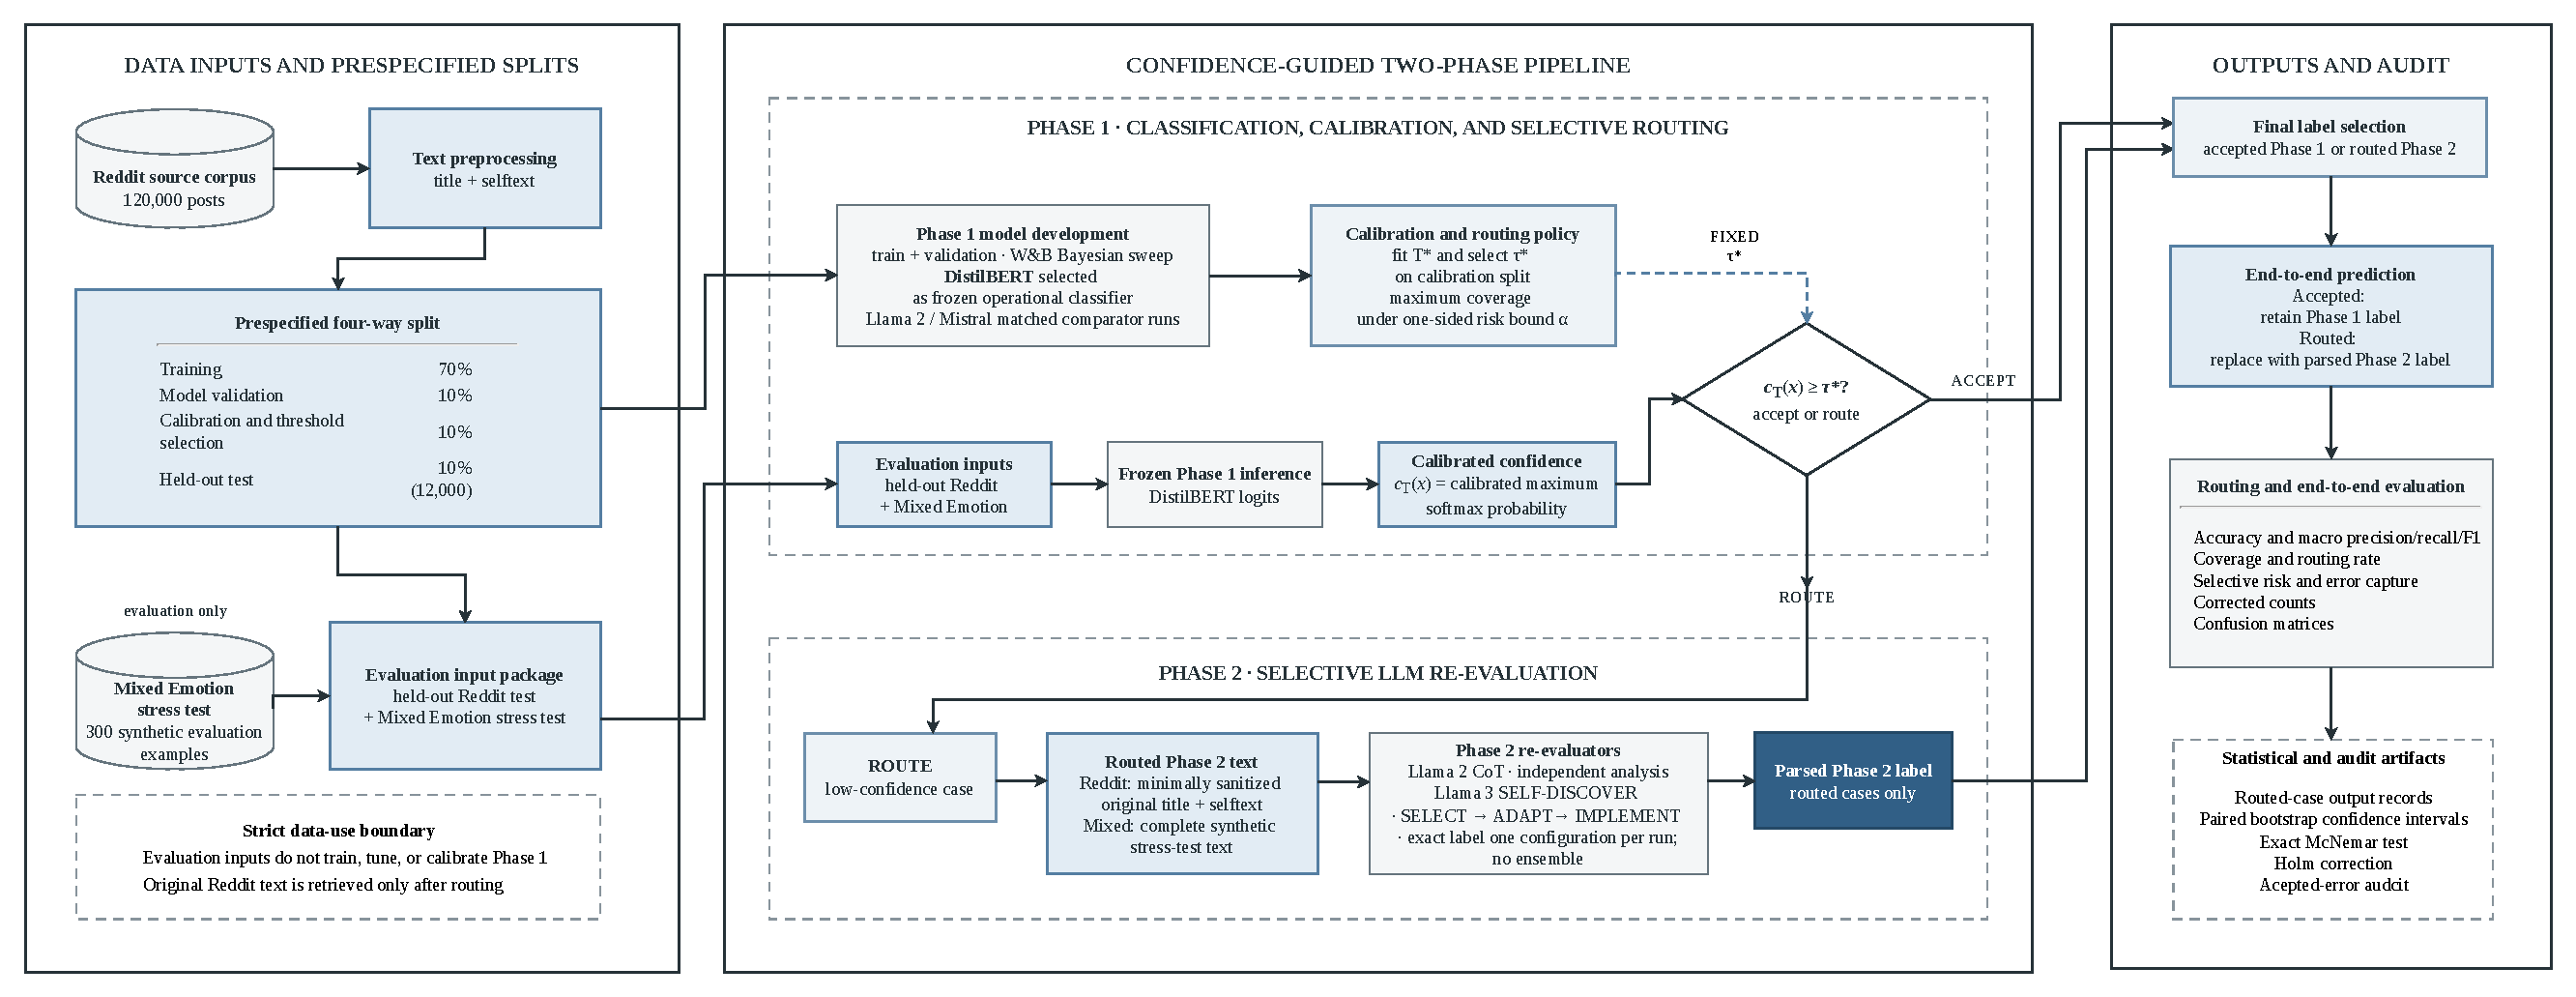
\includegraphics[width=\textwidth]{figures/architecture_figure_publication_final.pdf}
\caption{Confidence-guided two-phase pipeline. Accepted predictions retain the Phase 1 label, while routed posts enter re-evaluation. Original artwork is retained in this review copy pending label updates; the final experiment evaluates both models with Direct, CoT, and SELF-DISCOVER as specified in the text.}
\label{fig:architecture}
\end{figure*}
\subsection{Phase 1: Initial Emotion Classification}

The Phase~1 comparison includes DistilBERT \cite{ref12}, Mistral~7B \cite{ref13}, and Llama~2~7B \cite{ref14} under common data partitions and a four-trial search budget. DistilBERT is fully fine-tuned, whereas the 7B backbones use frozen representations with trainable linear heads. Thus, this is a comparison of practical classifier configurations, not an isolated test of architecture or maximum attainable performance. Each selected configuration is evaluated with seeds 42, 43, and 44. Appendix Table~A1c gives the selected settings; the final DistilBERT run under the selected configuration supplies downstream routing scores.

\subsection{DistilBERT}

DistilBERT \cite{ref12} is a compact bidirectional encoder obtained by distilling BERT into a six-layer student. Its original pretraining combines language-modeling, teacher-distribution matching, and representation-alignment objectives, producing a model with about 40\% fewer parameters than BERT-base and a reported inference speedup of about 60\% while retaining much of the teacher's language-understanding performance. Those properties make it an appropriate candidate for the high-volume first stage of a selective pipeline, where every input must be classified before only a small subset is escalated. In this study, the released \texttt{distilbert-base-uncased} checkpoint is fully fine-tuned with supervised three-class cross-entropy; the historical distillation process is not repeated. Its logits are subsequently temperature-calibrated, and only this operational checkpoint supplies the confidence scores used for routing.

\subsection{Mistral}

Mistral~7B \cite{ref13} is a decoder-only transformer with grouped-query attention (GQA) and sliding-window attention (SWA). GQA reduces key--value memory requirements, while SWA restricts attention to a local window. Here, Mistral provides a larger pretrained representation for three-class classification. Its backbone remains frozen, and a bias-free linear head maps the 4,096-dimensional representation to three class logits. Only the head's 12,288 parameters are trained; no adapter is added.

\subsection{Llama 2}

Llama~2 \cite{ref14} is a family of decoder-only autoregressive transformers. Its 7B base checkpoint supplies a second larger representation family for Phase~1 and is distinct from the chat-tuned checkpoint used in Phase~2. Classification uses the same frozen-backbone, bias-free 12,288-parameter linear-head design as Mistral. The shared partitions and label mapping permit predictive comparison, while the differing adaptation scope precludes attributing differences to model size alone.

All three classifiers output class logits. Post-hoc calibration and threshold selection are performed only for the operational DistilBERT checkpoint; no calibrated routing result is claimed for the comparison models.

\subsection{Calibrated Confidence-Based Routing and Risk-Coverage Threshold Selection}

The fixed operational DistilBERT classifier supplies the logits used for calibration and routing. For an input text $x_i$, it outputs logits $\mathbf{z}_i$ over $K$ proxy emotion classes. The uncalibrated class probability for class $k$ is computed with the softmax function:

\begin{equation}
p_{i,k}=\frac{\exp(z_{i,k})}{\sum_{j=1}^{K}\exp(z_{i,j})}.
\end{equation}

The Phase 1 predicted label is defined as:

\begin{equation}
\hat{y}_i = \arg\max_k p_{i,k}.
\end{equation}

Because raw maximum softmax probability may be poorly calibrated \cite{ref15}, a dedicated calibration split $D_{cal}$ is used to fit a scalar temperature parameter $T$. Temperature-scaled probabilities are computed as:

\begin{equation}
q_{i,k}(T)=
\frac{\exp(z_{i,k}/T)}
{\sum_{j=1}^{K}\exp(z_{i,j}/T)}.
\end{equation}

The temperature is selected by minimizing negative log-likelihood on $D_{cal}$:

\begin{equation}
T^*=\arg\min_{T>0}
\frac{1}{|D_{cal}|}\sum_{i\in D_{cal}} -\log q_{i,y_i}(T).
\label{eq:temperature-nll}
\end{equation}

NLL evaluates the probability assigned to the true class and penalizes confident mistakes strongly. Two complementary diagnostics are also reported. The multiclass Brier score measures the squared distance between the complete probability vector and the one-hot target vector:

\begin{equation}
\mathrm{Brier}(T)=\frac{1}{|D_{cal}|}
\sum_{i\in D_{cal}}\sum_{k=1}^{K}
\left(q_{i,k}(T)-\mathbf{1}[y_i=k]\right)^2.
\label{eq:brier}
\end{equation}

Expected calibration error (ECE) partitions predictions into confidence bins $B_m$ and compares mean confidence with empirical accuracy within each bin:

\begin{equation}
\mathrm{ECE}(T)=\sum_{m=1}^{M}\frac{|B_m|}{|D_{cal}|}
\left|\mathrm{acc}(B_m)-\mathrm{conf}(B_m)\right|.
\label{eq:ece}
\end{equation}

NLL, Brier score, and ECE are complementary rather than interchangeable selection constraints. NLL is the optimization objective for $T^*$; Brier score checks the quality of all class probabilities; and ECE checks whether stated confidence agrees with observed correctness at the group level. Adaptive ECE repeats the last comparison with approximately equal-frequency bins to reduce sensitivity to sparse fixed-width bins. Lower values are better for all four diagnostics.

The primary routing confidence score is then the temperature-scaled maximum softmax probability:

\begin{equation}
c_i=\max_k q_{i,k}(T^*).
\end{equation}

For a candidate routing threshold $\tau$, the accepted set $A(\tau)$ and routed set $R(\tau)$ are defined as:

\begin{align}
A(\tau) &= \{i: c_i \geq \tau\}, \\
R(\tau) &= \{i: c_i < \tau\}.
\end{align}

Coverage and routing rate are computed as:

\begin{align}
\mathrm{Coverage}(\tau) &= \frac{|A(\tau)|}{N}, \\
\mathrm{RoutingRate}(\tau) &= \frac{|R(\tau)|}{N} \\
&= 1-\mathrm{Coverage}(\tau).
\end{align}

Selective risk is computed only on accepted Phase 1 predictions:

\begin{equation}
\mathrm{Risk}(\tau)=
\frac{1}{|A(\tau)|}
\sum_{i \in A(\tau)}
\mathbf{1}[\hat{y}_i \ne y_i].
\end{equation}

To make the routing rule more conservative on finite calibration samples, the implementation also computes a one-sided binomial upper confidence bound $\overline{R}_{\delta}(\tau)$ for the accepted-set error rate using confidence level $1-\delta$. The final threshold is selected on $D_{cal}$ by maximizing coverage while satisfying the target selective-risk constraint $\alpha$:

Let $e(\tau)=\sum_{i\in A(\tau)}\mathbf{1}[\hat{y}_i\ne y_i]$ denote the number of accepted-set errors and $n(\tau)=|A(\tau)|$ denote the number of accepted examples. For $e(\tau)<n(\tau)$, the one-sided Clopper--Pearson upper bound used by the implementation is:

\begin{equation}
\overline{R}_{\delta}(\tau)=
\mathrm{Beta}^{-1}\!\left(
1-\delta;\,
e(\tau)+1,\,
n(\tau)-e(\tau)
\right),
\label{eq:clopper-pearson-bound}
\end{equation}

where $\mathrm{Beta}^{-1}(\cdot;a,b)$ is the inverse cumulative distribution function of a Beta$(a,b)$ distribution. When every accepted prediction is incorrect, the bound is set to 1; empty accepted sets are ineligible. The tail probability $\delta$ specifies the nominal confidence level, whereas $\alpha$ specifies the acceptable risk budget. This is a calibration-set selection criterion. Because temperature fitting and threshold search reuse the calibration data, pointwise Clopper--Pearson bounds do not establish a simultaneous post-selection guarantee for the resulting policy. Nor does the criterion guarantee risk control under distribution shift.

\begin{align}
\tau^* &= \arg\max_{\tau \in \mathcal{T}}
\mathrm{Coverage}(\tau) \\
\text{s.t.}\quad
\overline{R}_{\delta}(\tau) &\leq \alpha, \\
|A(\tau)| &\geq m_{\min}.
\end{align}

Here, $m_{\min}$ is a minimum accepted-sample requirement used to avoid selecting thresholds supported by too few calibration examples. The implementation sets $m_{\min}=\lceil0.10|D_{cal}|\rceil=1{,}200$. The selected $\tau=0.70$ accepted 11,807 calibration examples, so this safeguard was satisfied but did not determine the selected operating point. In the final DistilBERT operating policy, candidates are swept from 0.70 to 1.00 in increments of 0.01. This lower bound was chosen before held-out testing to avoid treating a weak three-class majority probability near 0.50 as sufficiently reliable for direct acceptance. Unless otherwise stated, the primary operating point uses temperature-scaled maximum softmax probability, a target selective risk of $\alpha=0.05$, a one-sided risk confidence level of $1-\delta=0.95$, the acceptance rule $c_i \geq \tau$, and the routing rule $c_i < \tau$. The risk constraint is a feasibility condition: it excludes candidate thresholds whose accepted-set upper risk exceeds $\alpha$. Among the feasible candidates in the prespecified 0.70--1.00 grid, the candidate with the greatest Phase~1 coverage is selected. Thus, the completed DistilBERT value $\tau^*=0.70$ reflects both the prespecified conservative operating range and calibration-set risk--coverage evaluation; it was not optimized using held-out test results or Phase~2 outcomes. The 7B models serve as Phase~1 predictive comparators only; they do not define alternative routing policies in the reported end-to-end experiment.

The threshold-selection output records accepted accuracy, routed Phase~1 errors, error capture, routing precision, and proxy-Depression false-negative risk among accepted predictions. Additional confidence diagnostics include expected calibration error (ECE), adaptive ECE, Brier score, and negative log-likelihood before and after temperature scaling. Auxiliary analyses compare raw MSP, temperature-scaled MSP, entropy-based certainty, and probability margin; estimate bootstrap confidence intervals for selective metrics; assess threshold stability through calibration-set resampling; and extract high-confidence accepted errors for qualitative auditing.

\begin{algorithm}[t]
\caption{Calibrated confidence-guided routing}
\label{alg:confidence-routing}
\footnotesize
\begin{algorithmic}[1]
\State \textbf{Input:} $D_{val}$, $D_{cal}$, classifier $f_{\theta}$
\State \textbf{Input:} $\alpha$, $1-\delta$, grid $\mathcal{T}$, minimum count $m_{\min}$
\State \textbf{Output:} temperature $T^*$ and threshold $\tau^*$
\State Select best checkpoint using $D_{val}$
\State Fit $T^*$ on $D_{cal}$ by minimizing NLL
\State Compute calibrated confidences $c_i$ on $D_{cal}$
\State Sweep the prespecified calibrated-confidence candidate grid
\For{each $\tau\in\mathcal{T}$}
    \State Form $A(\tau)$ and $R(\tau)$ from $c_i$
    \State Compute coverage, routing rate, and risk bound
\EndFor
\State Retain candidates with $\overline{R}_{\delta}(\tau)\leq\alpha$ and $|A(\tau)|\geq m_{\min}$
\State If none remain, flag infeasibility; a fallback is not risk-feasible
\State Choose a retained $\tau$ with maximum coverage
\State Fix $T^*$ and $\tau^*$ before held-out testing
\end{algorithmic}
\end{algorithm}

\begin{algorithm}[t]
\caption{Two-phase inference with fixed calibrated routing policy}
\label{alg:two-phase-inference}
\footnotesize
\begin{algorithmic}[1]
\State \textbf{Input:} post record $x$, classifier $f_{\theta}$, fixed $T^*$ and $\tau^*$
\State \textbf{Input:} Phase~2 configuration $g$ (model and prompting protocol)
\State Obtain the Phase~1 input $x^{(1)}$ from record $x$
\State Compute $\mathbf{z}=f_{\theta}(x^{(1)})$ and probabilities $q_k(T^*)$
\State Set $\hat{y}^{(1)}=\arg\max_k q_k(T^*)$ and $c=\max_k q_k(T^*)$
\If{$c \geq \tau^*$}
    \State \textbf{return} $\hat{y}^{(1)}$ as the accepted Phase~1 final label
\Else
    \State Retrieve the minimally sanitized original text $x^{(2)}$
    \State Generate a label with $g$ using its prescribed inputs
    \State Parse exactly one label from \{Depression, Neutral, Happy\}
    \State If parsing fails, retain $\hat{y}^{(1)}$ and record failure
    \State \textbf{return} the parsed label or recorded fallback
\EndIf
\end{algorithmic}
\end{algorithm}

\begin{algorithm}[t]
\caption{Audited end-to-end evaluation of routed predictions}
\label{alg:end-to-end-audit}
\footnotesize
\begin{algorithmic}[1]
\State \textbf{Input:} reference labels $y_i$, Phase~1 labels $\hat{y}^{(1)}_i$, route indicators $r_i$
\State \textbf{Input:} parsed Phase~2 labels $\hat{y}^{(2)}_i$ for routed inputs
\For{each example $i$}
    \State $\hat{y}^{(E)}_i \gets \hat{y}^{(2)}_i$ if $r_i=1$ and parsing succeeds; otherwise $\hat{y}^{(E)}_i \gets \hat{y}^{(1)}_i$
\EndFor
\State $C\gets\sum_i\mathbf{1}[r_i=1,\hat{y}^{(1)}_i\ne y_i,\hat{y}^{(E)}_i=y_i]$
\State $I\gets\sum_i\mathbf{1}[r_i=1,\hat{y}^{(1)}_i=y_i,\hat{y}^{(E)}_i\ne y_i]$
\State Report corrected errors $C$, introduced errors $I$, net corrections $C-I$
\State Report end-to-end metrics over all examples using $\hat{y}^{(E)}$
\end{algorithmic}
\end{algorithm}

Algorithm~\ref{alg:end-to-end-audit} formalizes the evaluation boundary between routed-subset behavior and full-set performance. In particular, a Phase~2 model is not credited merely for correcting selected errors: any newly introduced errors are deducted, and the final accuracy is recomputed over the complete evaluation set after accepted Phase~1 labels and routed Phase~2 labels are recombined.

The export notebook prints a warning and falls back to the lowest empirical risk, then highest coverage, if no candidate satisfies the constraint. That branch was not needed here: the selected calibration point satisfies the prescribed upper-bound criterion. A fallback, if invoked, would not be interpreted as a risk-feasible policy. The temperature, threshold, risk target, confidence level, and candidate grid are stored with the calibration and threshold tables. The model source and seed are recorded separately in the execution environment artifact.

\subsection{Relationship to Mixed-Emotion Evaluation}

The routing mechanism is entirely confidence-based during inference. It does not directly detect blended emotion or sentiment shift. Instead, the Mixed Emotion Dataset serves a complementary evaluation role by stress-testing whether the Phase 1 classifier and the Phase 2 reasoning stage behave more reliably on examples where the one-label-per-input assumption is more difficult. This separation keeps the routing rule reproducible while allowing the evaluation to probe emotionally complex cases.

\begin{figure*}[t]
\centering
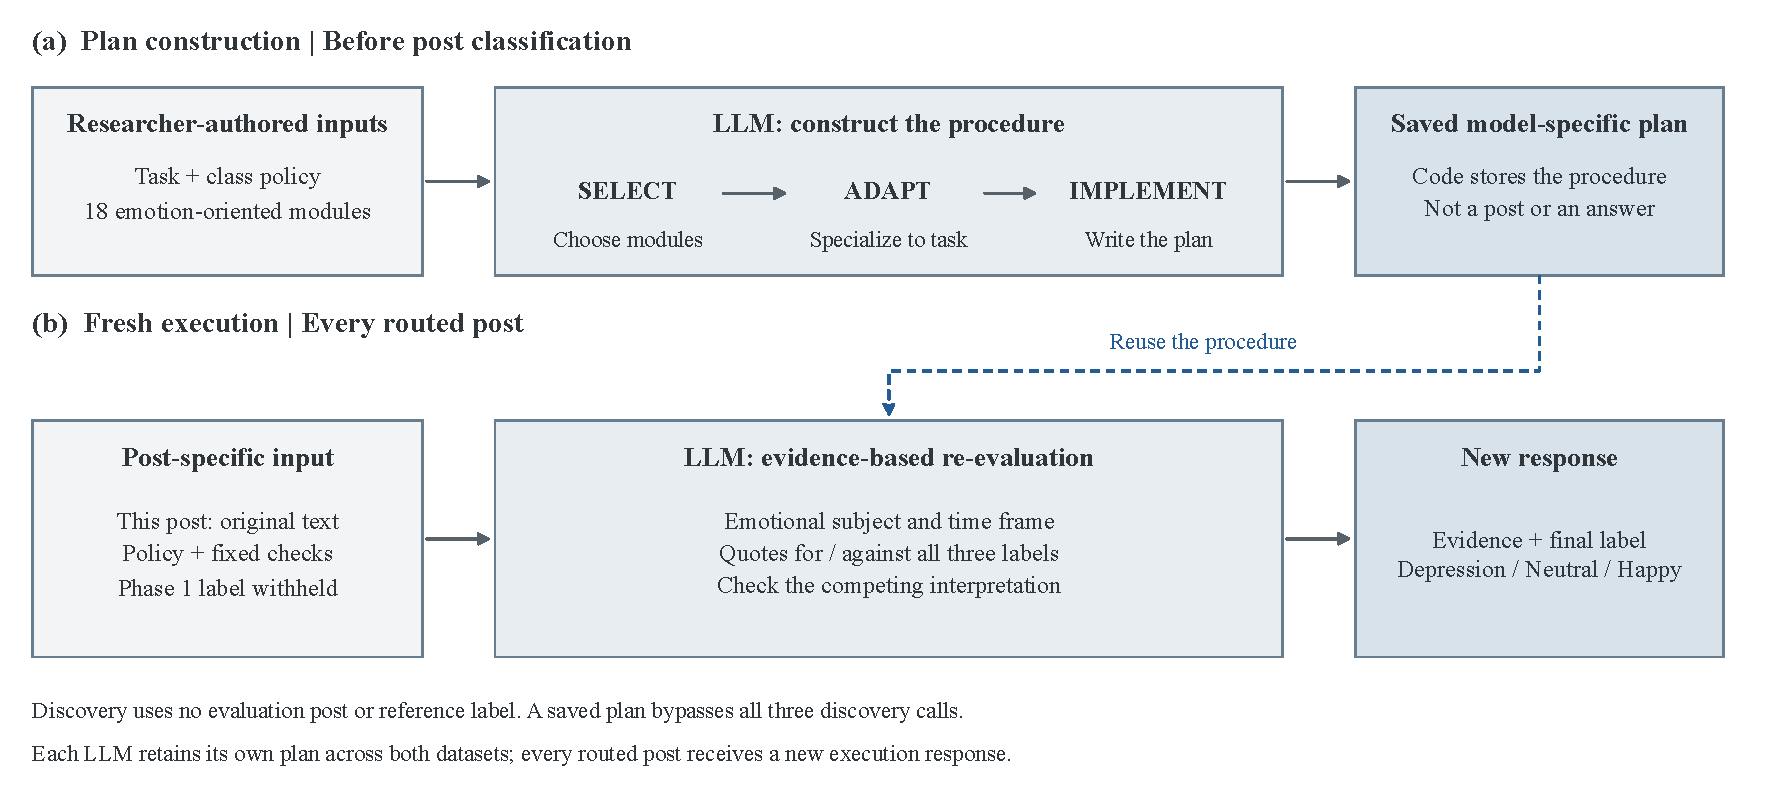
\includegraphics[width=\textwidth]{figures/sd_task_level_overview.pdf}
\caption{Task-specific SELF-DISCOVER design within selective re-evaluation. (a) Before post classification, the selected LLM constructs a model-specific procedure from researcher-authored task materials; the code saves it for reuse. (b) Each routed original post is evaluated anew using that procedure and fixed subject, time-frame, evidence, and alternative-interpretation checks. The dashed arrow denotes procedure reuse, not answer reuse. Discovery is skipped when a retained plan exists. Appendix~\ref{app:sd-templates} provides the detailed workflow and exact prompts; label parsing and Phase~1 fallback follow Algorithm~\ref{alg:sd-final}.}
\label{fig:sd-task-level}
\end{figure*}

\subsection{Phase 2: Factorial Model and Protocol Comparison}
Direct prompting requests one final label without a rationale and includes the Phase~1 prediction. CoT first requests an independent assessment, subsequently discloses the Phase~1 label for comparison, and finally requests a terminal label. The implemented CoT dialogue contains five generation calls, including the initial acknowledgment and text-response turns. Final SELF-DISCOVER withholds the Phase~1 label throughout. These are complete prompting protocols: their comparison does not isolate rationale length alone, because label disclosure and call structure also differ.

\subsection{Task-Level SELF-DISCOVER}
SELF-DISCOVER separates \emph{constructing a procedure} from \emph{applying it}, as summarized in Figure~\ref{fig:sd-task-level}. Each model generates a plan for the three-class task, stores it, and reuses it across routed posts. This \emph{cached plan} is a saved procedure, not stored post-level answers. Every post still requires a new model response.

\textit{Task-specific design.} We retain the SELECT--ADAPT--IMPLEMENT framework of SELF-DISCOVER \cite{ref18} and specialize its inputs and execution guidance to proxy emotion classification. Researchers supply the class policy, 18 emotion-oriented reasoning modules, and fixed evidence-checking instructions; the LLM generates the procedure from those materials. The adaptation addresses distinctions that isolated affect words cannot resolve: whose emotion is expressed, whether distress is current or retrospectively resolved, and whether positive wording describes an actual state rather than a wish. The contribution is this task-specific specification and its integration with selective re-evaluation, not the invention of task-level planning or caching.

\textit{Who constructs the plan, and when.} Before classifying a routed post, the code checks for a retained plan for the selected LLM. If none exists, that LLM receives only the researcher-authored task description, policy, and module bank. It does not receive the first post, any other evaluation post, a reference label, or a Phase~1 prediction during discovery. SELECT chooses relevant modules; ADAPT specializes them to the task; IMPLEMENT generates the reusable procedure, which the code stores. If a plan already exists, all three discovery calls are skipped. Llama~2 and Llama~3 generate separate plans; each model reuses its own plan across Reddit and Mixed Emotion.

IMPLEMENT requests at most three one-line JSON steps, each returning to the original text and deferring label selection until the end. This format is requested, not enforced; the realized plans are reproduced in Appendix~\ref{app:sd-templates}. Access to the post is an instruction for subsequent execution, not an input to plan construction.

\textit{Per-post execution.} The prompt combines the plan, policy, original post, and fixed checks. It asks whose emotion is expressed, whether it is current or retrospectively resolved, and which quotations support or oppose each label. A counterfactual check asks what evidence would favor the second-best label and whether it is present. The model emits a final classification line. SD never receives the Phase~1 label; the evaluator retains it as a fallback if parsing fails.

This division keeps the procedure shared while requiring fresh, post-specific evidence and a new decision for every routed input. The evidence ledger and counterfactual check are researcher-authored execution instructions, not automatically discovered properties of the cached plan. Generated explanations do not establish faithful internal reasoning. Appendix~\ref{app:sd-templates} provides the workflow, templates, and actual plans; Appendix~\ref{app:sd-variants} compares the earlier per-post and final task-level designs without attributing their differences to any single component.

\begin{algorithm}[t]
\caption{Final task-level SELF-DISCOVER re-evaluation}
\label{alg:sd-final}\footnotesize
\begin{algorithmic}[1]
\State \textbf{Input:} model $g$; researcher-authored task, policy, modules, execution guidance; routed posts
\If{a retained plan for $g$ exists}
\State Load that plan; skip discovery
\Else
\State Give $g$ task materials only; no post text or labels
\State $g$: SELECT relevant modules and ADAPT them to the task
\State $g$: IMPLEMENT the procedure; store it as the plan
\EndIf
\For{each routed post $x$}
\State Execute the plan on the original post, without the Phase~1 label
\State Request source quotes, three-label evidence, and a counterfactual check
\State Parse the final label; retain Phase~1 if parsing fails
\State Store the response, parsed status, and final prediction
\EndFor
\end{algorithmic}\end{algorithm}

\subsection{Input and Output Policy}
Reddit Phase~1 uses cleaned title--body text; Phase~2 uses the linked, minimally sanitized original title and selftext. The original-text policy preserves punctuation, negation, and discourse structure but changes the input representation as well as the prediction mechanism. Improvements are therefore attributed to the complete re-evaluation configuration, not solely to reasoning. Long posts follow the notebook's 6,000-character input policy. Mixed Emotion uses the complete synthetic text rather than a separately lemmatized version.

The three permitted outputs are Depression, Neutral, and Happy. The parser prioritizes the terminal label marker and records unparseable responses. Such responses retain the Phase~1 prediction in the end-to-end evaluation; parsing failure is not automatically counted as a classification error. The remaining final SELF-DISCOVER failures are not regenerated or assigned labels from the reference answer. Label normalization and any recovery of an explicit answer must be applied without consulting the reference label.
\section{Experimental Setup}
\subsection{Classifier Selection and Calibration}
All classifier configurations use the common 84,000/12,000/12,000/12,000 train/validation/calibration/test partitions, a maximum length of 256 tokens, and a four-trial Bayesian search maximizing validation macro F1. The selected DistilBERT settings are learning rate $4.0368\times10^{-5}$, batch size 64, an epoch budget of 3, and weight decay $10^{-3}$. The epoch budget is a selected training hyperparameter, not a statement that every seed's best validation checkpoint occurred at that epoch. Seeds 42, 43, and 44 characterize classifier variation; the final downstream run uses seed 42. Appendix Table~A1c records the selected settings for all three classifiers.

The downstream export loads the saved reference seed-42 model from this selected configuration; it does not perform a new training run inside the export notebook. Its environment record identifies fp32 evaluation, a 256-token maximum input length, and the same selected hyperparameters. The final model is calibrated with $T^*=1.480195$ and routed at $\tau^*=0.70$. The calibration partition has 11,807 accepted and 193 routed posts, accepted-set empirical risk 1.9395\%, and one-sided upper bound 2.1615\%, below the 5\% target. These calibration counts are distinct from the 218 routed Reddit test posts. No Mixed Emotion labels are used for temperature fitting or threshold selection.

\subsection{Execution and Resource Scope}
The retained Phase~1 benchmark compares the selected classifier configurations on NVIDIA A100-SXM4-40GB hardware, with fp16 inference, a 256-token cap, and batch size 32. Three timing repetitions are distinct from the three training seeds. These classifier-stage measurements are not measurements of the complete final reasoning pipeline; Appendix Table~A1d retains their original measurement scope.

Phase~2 uses chat-tuned Llama~2~7B and instruction-tuned Llama~3~8B with quantized loading and greedy decoding. Direct and final CoT request up to 1,024 new tokens per call. Final SELF-DISCOVER requests up to 1,024 for Llama~2 and 1,536 for Llama~3 in its per-post execution call. Thus, neither total generation cost nor token budget is claimed to be equal across all protocols. Llama~2's shorter context also constrains multi-turn inference. Template text and nominal execution budgets are disclosed in the appendices; wall-clock or monetary superiority of the final Phase~2 configurations is not inferred from accuracy.

\subsection{Evaluation and Statistical Scope}
Accuracy and macro F1 use all examples, after recombining accepted and routed predictions. Corrected errors $C$ are Phase~1 mistakes made correct by re-evaluation; introduced errors $I$ are previously correct predictions made wrong. The full-set accuracy change in percentage points is $100(C-I)/N$. Wrong-to-wrong changes are not corrections. Routed accuracy, error capture, and accepted-set risk measure different aspects of the pipeline.

Appendix~\ref{app:statistics} reports count-based paired accuracy summaries. For a comparison with Phase~1, the discordant pairs are exactly $C$ and $I$, so the two-sided exact McNemar test is a binomial test with $C+I$ trials and probability one half. Paired percentile-bootstrap intervals for accuracy change are reconstructed from the three correctness-difference categories $+1,-1,0$, with counts $C,I,N-C-I$, using 50,000 multinomial resamples. This is equivalent to a paired row bootstrap for that scalar accuracy difference. It does not reconstruct class-wise metrics or paired comparisons between two re-evaluators. Holm correction is applied across the 12 final configuration-versus-Phase~1 tests. These intervals and tests describe the reported final counts; prompt development and selection make them exploratory rather than selection-adjusted confirmation of the winning prompt.
\section{Experimental Results}
\subsection{Phase 1 Performance on Reddit Data}

The matched Phase~1 comparison used the same class-balanced 120,000-post sample, prespecified 70/10/10/10 partitions, 12,000-example held-out test set, maximum input length of 256 tokens, four-trial Bayesian search budget, and random seeds 42, 43, and 44 for all three architectures. Table~\ref{tab:phase1-performance} reports predictive performance and inference efficiency for these configurations; training configurations are documented in Appendix Table~A1c.

\begin{table*}[t]
\centering
\caption{Matched Phase~1 predictive performance and inference efficiency}
\label{tab:phase1-performance}
\footnotesize
\setlength{\tabcolsep}{4.2pt}
\renewcommand{\arraystretch}{1.16}
\textbf{(a) Predictive performance on the common 12,000-post test set}\par\smallskip
\begin{tabularx}{\textwidth}{@{}l *{4}{>{\centering\arraybackslash}X}@{}}
\toprule
Model & Accuracy, mean $\pm$ SD & Accuracy 95\% CI & Macro F1, mean $\pm$ SD & Macro F1 95\% CI \\
\midrule
DistilBERT & 96.88 $\pm$ 0.04\% & [96.79, 96.98]\% & 96.88 $\pm$ 0.04\% & [96.79, 96.98]\% \\
Mistral~7B & 95.36 $\pm$ 0.08\% & [95.15, 95.57]\% & 95.36 $\pm$ 0.08\% & [95.16, 95.56]\% \\
Llama~2~7B & 95.17 $\pm$ 0.07\% & [95.00, 95.34]\% & 95.17 $\pm$ 0.07\% & [94.99, 95.34]\% \\
\bottomrule
\end{tabularx}
\vspace{2pt}
\parbox{\textwidth}{\footnotesize \textit{Note.} Panel (a) reports percentages over training seeds 42, 43, and 44. Confidence intervals are two-sided Student-$t$ intervals across the three seed-level results. The comparison evaluates a bounded operational screening protocol; it does not estimate fully tuned 7B performance.}
\par\medskip
\textbf{(b) Inference on NVIDIA A100-SXM4-40GB}\par\smallskip
\begin{tabularx}{\textwidth}{@{}l >{\centering\arraybackslash}X >{\centering\arraybackslash}X >{\centering\arraybackslash}X@{}}
\toprule
Model & Throughput (posts/s) & Single-post p50 (ms) & Peak memory (GB) \\
\midrule
DistilBERT & 4,959.5 $\pm$ 15.5 & 4.80 $\pm$ 0.03 & 0.29 \\
Mistral~7B & 51.7 $\pm$ 0.0 & 36.62 $\pm$ 0.06 & 15.22 \\
Llama~2~7B & 55.5 $\pm$ 0.0 & 34.05 $\pm$ 0.10 & 14.05 \\
\bottomrule
\end{tabularx}
\par\smallskip
\parbox{\textwidth}{\footnotesize \textit{Note.} Panel (b) reports mean $\pm$ SD across three timing repetitions, distinct from the training seeds in panel (a). Throughput uses batch size 32 and all 12,000 test posts; p50 is the median latency for 512 posts processed individually. All models use fp16 and a 256-token cap. Memory refers to batched inference. An SD displayed as 0.0 reflects rounding. Appendix Table~A1d provides p95 latency and the full protocol.}
\end{table*}

Figure~\ref{fig:phase1-model-comparison} visualizes the same observed three-seed results and their 95\% confidence intervals. DistilBERT achieved 96.88 $\pm$ 0.04\% accuracy, compared with 95.36 $\pm$ 0.08\% for Mistral and 95.17 $\pm$ 0.07\% for Llama~2. Macro F1 showed the same pattern. Under this fixed comparison protocol, DistilBERT exceeded Mistral and Llama~2 by 1.52 and 1.71 percentage points in mean accuracy, respectively. The two probes differed by 0.19 points; their relative ordering is not the basis of the operational choice.

\begin{figure*}[t]
\centering
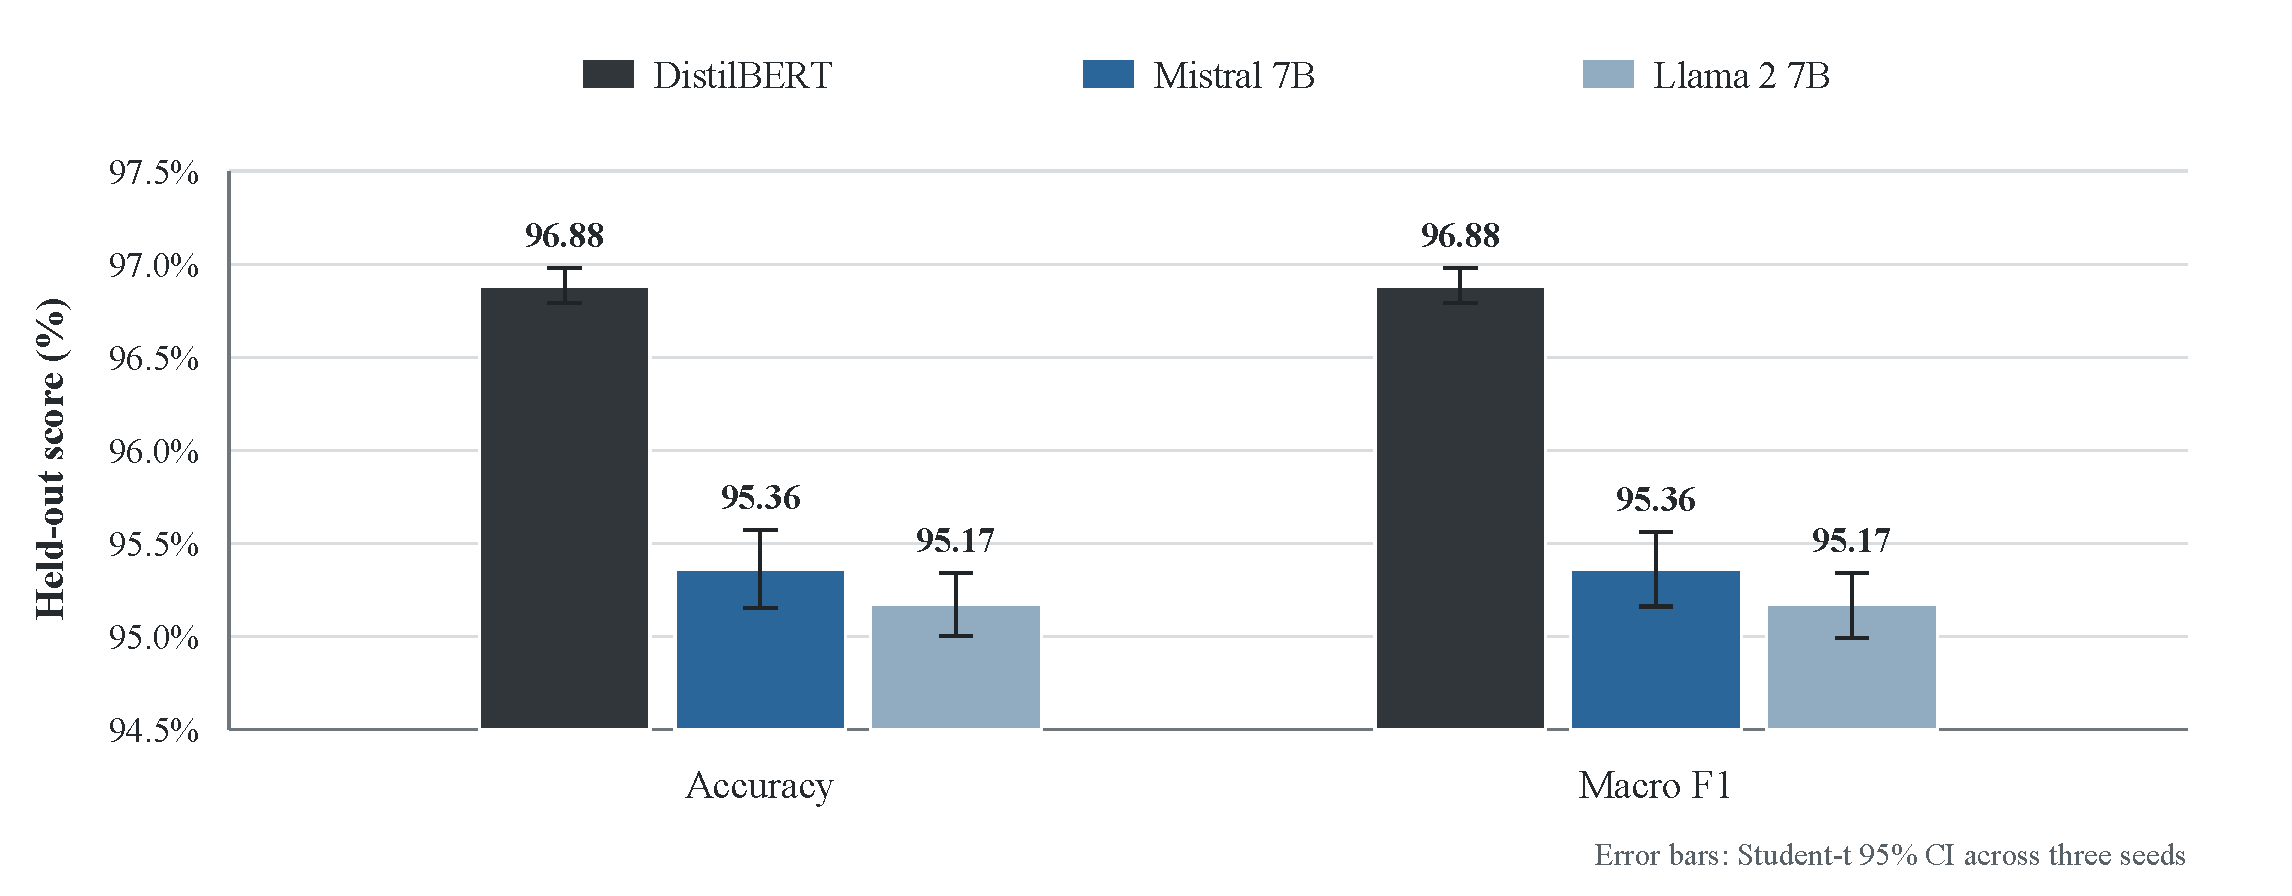
\includegraphics[width=0.88\textwidth]{figures/figure_e_phase1_model_comparison.pdf}
\caption{Observed Phase~1 classifier performance on the common 12,000-example held-out Reddit test set. Columns show three-seed means and whiskers show Student-$t$ 95\% confidence intervals for accuracy and macro F1. These intervals describe training-run variation, not repeated timing measurements. The vertical axis is truncated to make the between-model differences legible.}
\label{fig:phase1-model-comparison}
\end{figure*}

DistilBERT had the highest mean score and approximately 67 million parameters, compared with about seven billion for each comparator. These results support retaining it for the tested pipeline, without establishing superiority over fully adapted 7B models. Depression--Happy confusions accounted for 72.8\% of DistilBERT errors, 75.6\% of Llama~2 errors, and 74.3\% of Mistral errors across pooled seed predictions; Neutral F1 exceeded 98\% for all three. Pooling summarizes error composition, not 36,000 independent test examples. Small probe seed deviations also reflect the frozen backbone and should not be interpreted as equivalent training variability across adaptation methods.


The final linked DistilBERT run achieves 96.9167\% accuracy and 96.9166\% macro F1 on Reddit. This run uses the same selected hyperparameter configuration as the three-seed comparison. Its calibration and routing outputs, rather than those of a separately configured model, define every downstream condition.
\subsection{Class-Level Error Structure}
Figure~\ref{fig:phase1-confusion} shows the final linked classifier's errors on both datasets. Cell counts and row-normalized percentages distinguish the balanced Reddit test from the smaller stress test. These are the final Phase~1 predictions, not pooled three-seed counts or re-evaluation outputs.
\begin{figure*}[t]
\centering
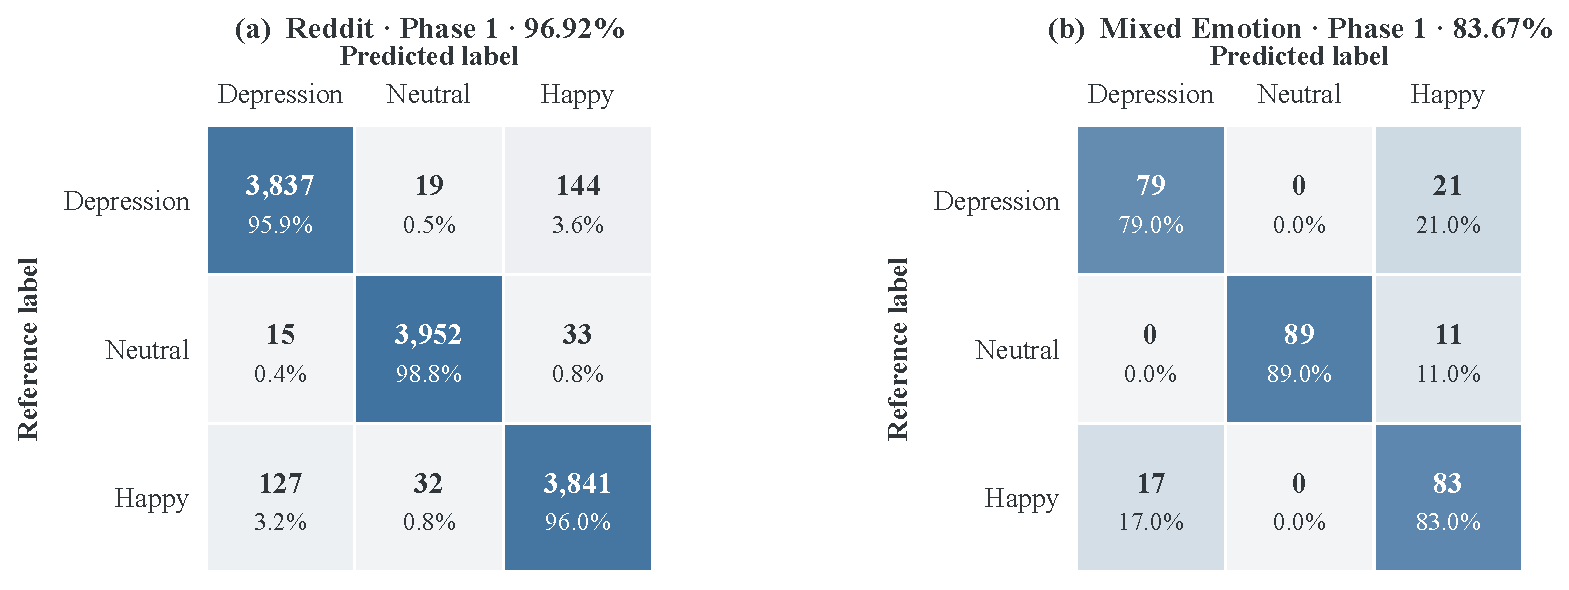
\includegraphics[width=0.96\textwidth]{figures/phase1_confusion.pdf}
\caption{Final Phase 1 confusion matrices on Reddit ($N=12{,}000$) and Mixed Emotion ($N=300$). Rows are reference labels; columns are predictions. Each cell shows a count and its percentage within the reference class. Both panels use the same row-normalized color scale.}
\label{fig:phase1-confusion}
\end{figure*}

\subsection{Calibration and Routing}
Temperature scaling reduces all four calibration diagnostics (Table~\ref{tab:calibration-final}). The fixed test router selects 218 of 12,000 Reddit posts and 86 of 300 Mixed Emotion examples. The difference in routing volume is an observed response to the stress-test inputs, not a dataset-specific threshold adjustment.
\begin{table*}[t]
\centering\small
\setlength{\tabcolsep}{4pt}\renewcommand{\arraystretch}{1.14}
\caption{Final DistilBERT calibration diagnostics (calibration split)}
\label{tab:calibration-final}
\begin{tabular*}{\textwidth}{@{\extracolsep{\fill}}lrrrrr@{}}
\toprule
Score & Temperature & NLL & Brier & ECE & Adaptive ECE \\
\midrule
Raw MSP & 1.0000 & 0.0933 & 0.0443 & 0.0176 & 0.0171 \\
Temperature-scaled MSP & 1.4802 & 0.0795 & 0.0416 & 0.0064 & 0.0128 \\
\bottomrule
\end{tabular*}
\end{table*}

\begin{figure*}[t]\centering
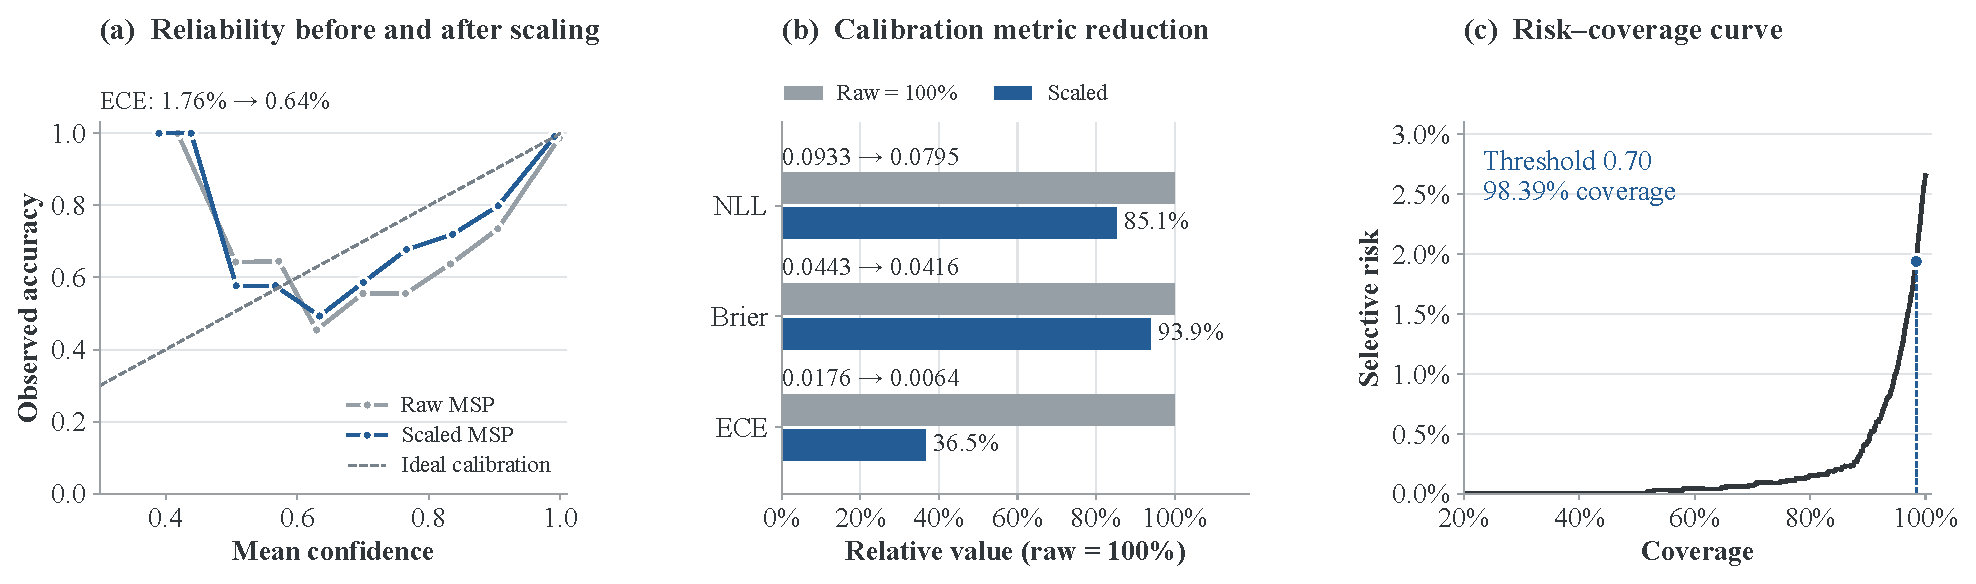
\includegraphics[width=\textwidth]{figures/calibration.pdf}
\caption{Calibration diagnostics for the final linked DistilBERT model. Reliability, relative metric reduction, and risk--coverage curves use the calibration split; the selected point is not selected on test outcomes.}
\label{fig:calibration-final}
\end{figure*}
\begin{table*}[t]
\centering\small
\setlength{\tabcolsep}{4pt}\renewcommand{\arraystretch}{1.14}
\caption{Fixed-policy routing outcomes; rates are percentages}
\label{tab:routing-final}
\begin{tabular*}{\textwidth}{@{\extracolsep{\fill}}lrrrrrrr@{}}
\toprule
Dataset & $N$ & Routed & Route rate & Coverage & Error capture & Routed error & Accepted risk \\
\midrule
Reddit & 12000 & 218 & 1.82 & 98.18 & 26.49 & 44.95 & 2.31 \\
Mixed Emotion & 300 & 86 & 28.67 & 71.33 & 57.14 & 32.56 & 9.81 \\
\bottomrule
\end{tabular*}
\end{table*}

On Reddit, the routed subset contains 98 of the 370 Phase~1 errors (26.49\% error capture). Its error rate is 44.95\%, compared with 3.08\% over the full set, an approximately 14.58-fold enrichment. The accepted subset still contains 272 errors, beyond the scope of routed-only correction. On Mixed Emotion, routing captures 28 of 49 errors (57.14\%); 21 errors remain accepted. Routed-set Phase~1 accuracy is 55.05\% on Reddit and 67.44\% on Mixed Emotion.

\begin{figure*}[t]
\centering
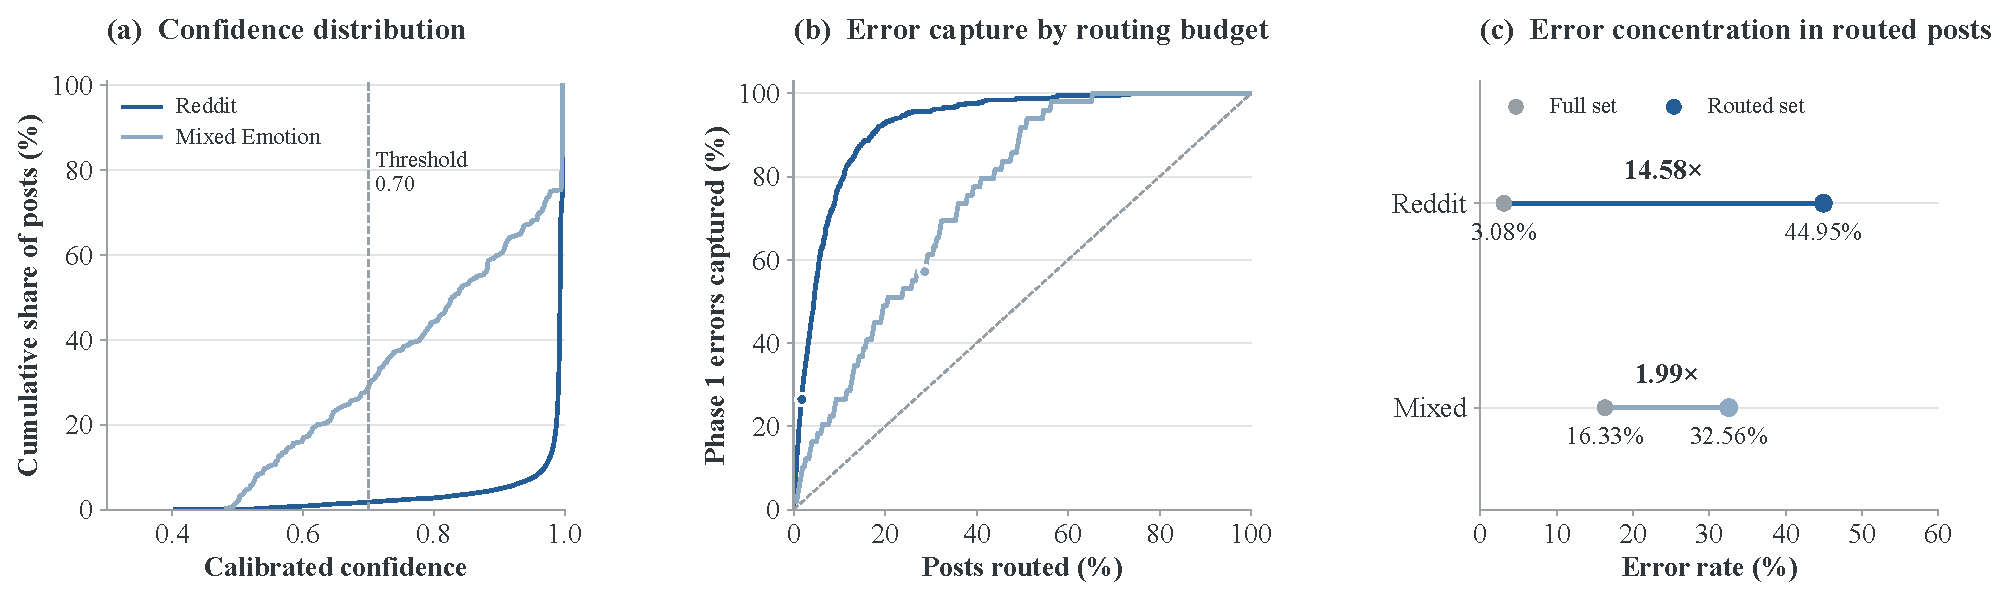
\includegraphics[width=\textwidth]{figures/routing_concentration.pdf}
\caption{Fixed-policy routing concentration. (a) Cumulative calibrated-confidence distributions. (b) Errors captured when posts are ordered from lowest to highest confidence; dots identify the fixed threshold and the diagonal is a proportional-capture reference. (c) Full-set and routed error rates, with enrichment ratios. Curves describe the evaluation sets; they are not used to select the threshold.}
\label{fig:routing-concentration}
\end{figure*}

\subsection{End-to-End Model and Prompting Results}
Table~\ref{tab:final-e2e} reports the complete final comparison. Llama~3 SELF-DISCOVER has the highest observed accuracy and macro F1 among these six configurations on both datasets. The advantage over Llama~3 CoT on Reddit is six correct predictions (0.0500 percentage points); numerical ordering alone does not establish a significant between-method difference.
\begin{table*}[t]
\centering\small
\setlength{\tabcolsep}{4pt}\renewcommand{\arraystretch}{1.14}
\caption{Final full-set outcomes on 12,000 Reddit posts and 300 Mixed Emotion examples. Accuracy and macro F1 are percentages; change is relative to Phase 1 in percentage points. $C$ counts corrected errors and $I$ newly introduced errors; $C-I$ is their net difference. Unparsed responses retain Phase 1 predictions.}
\label{tab:final-e2e}
\begin{tabular*}{\textwidth}{@{\extracolsep{\fill}}lllrrrrrr@{}}
\toprule
Dataset & Model & Protocol & Accuracy & Macro F1 & $C$ & $I$ & $C-I$ & Change \\
\midrule
Reddit & DistilBERT & Phase 1 & 96.9167 & 96.9166 & -- & -- & -- & -- \\
Reddit & Llama 2 & Direct & 96.9917 & 96.9898 & 45 & 36 & +9 & +0.0750 \\
Reddit & Llama 2 & CoT & 96.9250 & 96.9240 & 48 & 47 & +1 & +0.0083 \\
Reddit & Llama 2 & SELF-DISCOVER & 96.9417 & 96.9391 & 52 & 49 & +3 & +0.0250 \\
Reddit & Llama 3 & Direct & 97.1083 & 97.1056 & 68 & 45 & +23 & +0.1917 \\
Reddit & Llama 3 & CoT & 97.1500 & 97.1471 & 63 & 35 & +28 & +0.2333 \\
Reddit & Llama 3 & SELF-DISCOVER & 97.2000 & 97.1990 & 72 & 38 & +34 & +0.2833 \\
Mixed Emotion & DistilBERT & Phase 1 & 83.6667 & 84.0005 & -- & -- & -- & -- \\
Mixed Emotion & Llama 2 & Direct & 76.3333 & 75.1627 & 11 & 33 & -22 & -7.3333 \\
Mixed Emotion & Llama 2 & CoT & 79.0000 & 78.9298 & 19 & 33 & -14 & -4.6667 \\
Mixed Emotion & Llama 2 & SELF-DISCOVER & 89.3333 & 89.3452 & 22 & 5 & +17 & +5.6667 \\
Mixed Emotion & Llama 3 & Direct & 89.3333 & 89.3803 & 26 & 9 & +17 & +5.6667 \\
Mixed Emotion & Llama 3 & CoT & 84.6667 & 84.6760 & 15 & 12 & +3 & +1.0000 \\
Mixed Emotion & Llama 3 & SELF-DISCOVER & 92.6667 & 92.6966 & 28 & 1 & +27 & +9.0000 \\
\bottomrule
\end{tabular*}
\end{table*}

\begin{figure*}[t]\centering
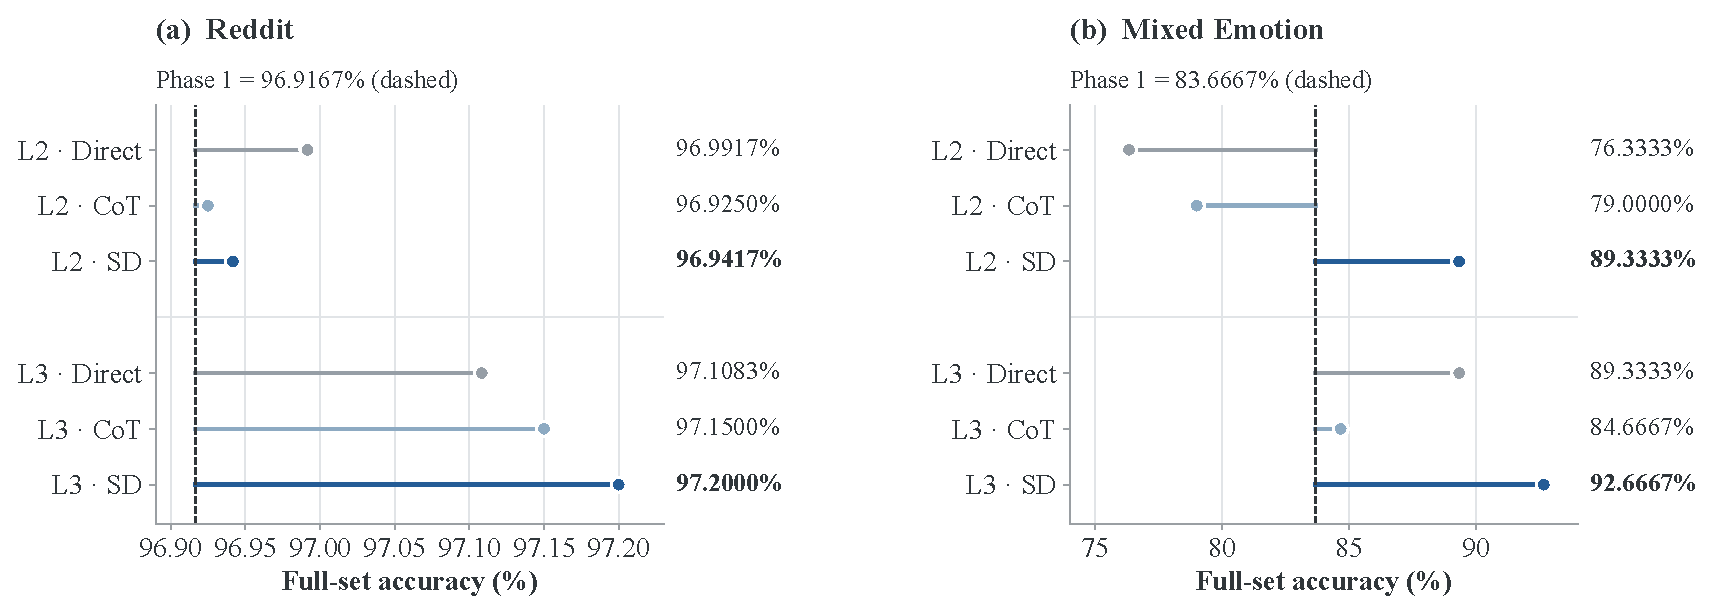
\includegraphics[width=\textwidth]{figures/end_to_end.pdf}
\caption{Full-set accuracy for the final six configurations. Points show observed accuracy; horizontal segments connect each point to the linked Phase 1 baseline (dashed line). The two panels use different axis ranges. SD denotes the final task-level compact-plan SELF-DISCOVER protocol.}
\label{fig:final-effect}
\end{figure*}

\subsection{Correction and Harm}
On Reddit, Llama~3 SELF-DISCOVER corrects 72 errors and introduces 38, producing 34 net corrections. Direct and CoT yield 23 and 28 net corrections, respectively. Llama~2 yields smaller gains: Direct has nine net corrections, CoT one, and SELF-DISCOVER three. Thus, SELF-DISCOVER does not outperform Direct within every model and dataset combination.

On Mixed Emotion, Llama~3 SELF-DISCOVER corrects 28 errors and introduces one. Total errors decrease from 49 to 22, a 55.10\% relative reduction, and accuracy increases by 9.00 percentage points. This low introduced-error count is an observed property of the 300-example stress test, not a population safety guarantee. Llama~2 SELF-DISCOVER also improves the baseline (17 net corrections), whereas its Direct and CoT configurations introduce more errors than they correct. The pattern supports evaluating both correction yield and damage to initially correct predictions.

\begin{figure*}[t]\centering
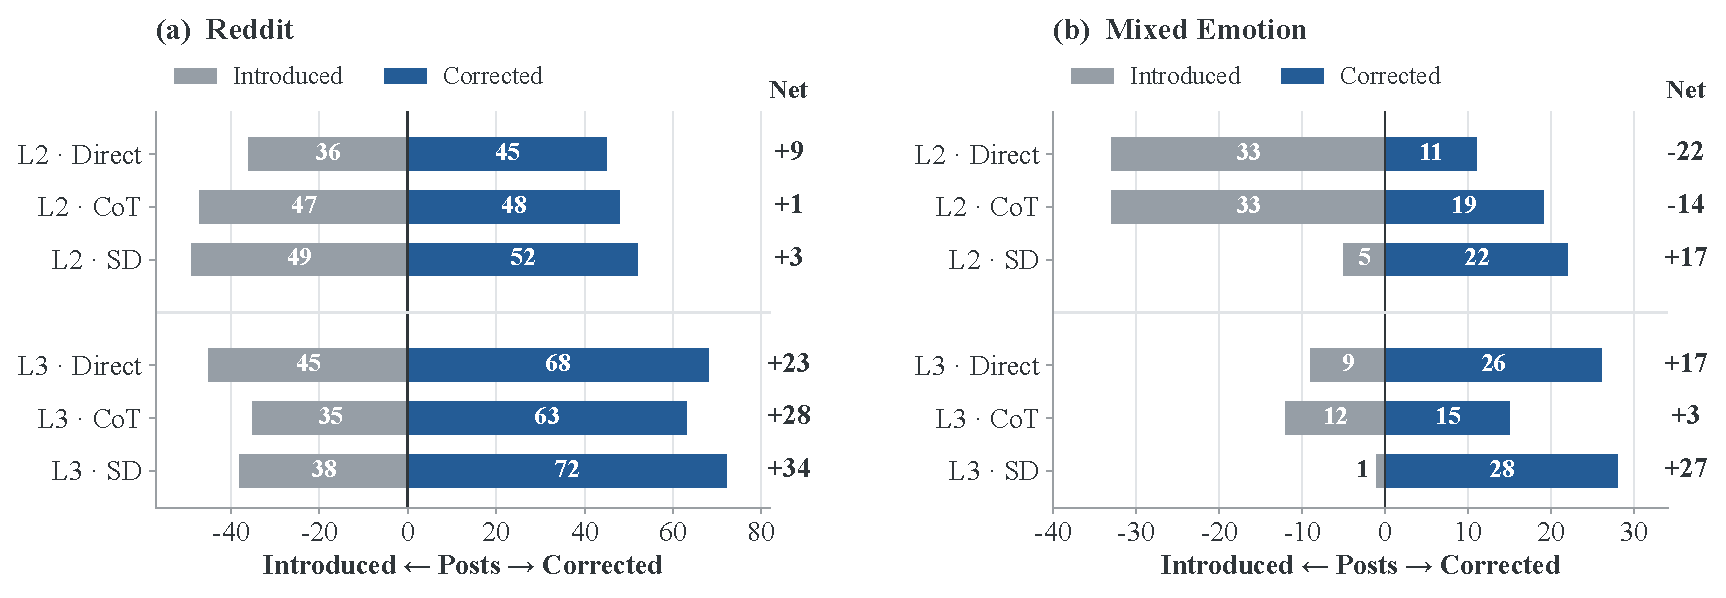
\includegraphics[width=\textwidth]{figures/corrections.pdf}
\caption{Corrected (blue, right) and introduced (gray, left) errors for each final configuration. Introduced counts are plotted to the left for comparison, not as negative error counts. Right-hand labels show net corrections. The panels use different count scales.}
\label{fig:final-errors}
\end{figure*}

\subsection{Conditional Correction Opportunity}
With the router held fixed, a conditional oracle corrects every routed error without changing any initially correct prediction. Its full-set ceiling is $\mathrm{Acc}_{P1}+E_R/N$, where $E_R$ is the number of routed Phase~1 errors. The ceiling is 97.7333\% on Reddit and 93.0000\% on Mixed Emotion. Final Llama~3 SELF-DISCOVER realizes $34/98=34.69\%$ and $27/28=96.43\%$ of these respective net-correction opportunities. These are descriptive ceilings under a fixed router, not achievable performance guarantees or alternative tuned baselines.
\Needspace{6\baselineskip}
\section{Discussion}
\subsection{An Efficient First Stage and a Selective Second Stage}
The linked experiment separates three decisions: selecting a practical classifier, routing uncertain posts, and choosing a re-evaluation protocol. DistilBERT retains strong three-seed predictive performance and a measured classifier-stage inference advantage under the bounded Phase~1 comparison. The final run then supplies one consistent set of predictions and confidence scores for every Phase~2 condition. Classifier means and downstream single-run scores answer different questions without requiring different hyperparameter configurations.

\subsection{Selection and Correction Are Different Outcomes}
Confidence routing identifies an error-enriched subset, but enrichment alone is insufficient. Llama~2 CoT is nearly neutral on Reddit and harmful on Mixed Emotion, whereas final SELF-DISCOVER with Llama~3 improves both sets. On the stress test, searching for evidence for and against all three classes and distinguishing present distress from resolved or attributed events are plausible contributors to the observed pattern. The experiment evaluates the complete prompt package; it does not establish the separate causal effect of each instruction or demonstrate that the generated rationale faithfully reveals the model's computation.

\subsection{What the Model--Protocol Comparison Shows}
Llama~3 SELF-DISCOVER has the highest observed accuracy and macro F1 on both sets. However, the 0.2833-point Reddit gain uses a 1.82\% routing rate, whereas the 9.00-point Mixed Emotion gain uses 28.67\%. These are different correction opportunities, not directly comparable effect sizes. Likewise, one introduced stress-test error versus 38 Reddit errors warrants dataset-specific interpretation rather than a universal reliability claim.

The methodological value of the adaptation is to specify what evidence a selected post should be checked against, rather than merely requesting a longer explanation. Emotional subject and time-frame checks address attribution and trajectory, while the three-label ledger and counterfactual check make competing interpretations explicit. The observed gains support this complete configuration within the evaluated settings; they do not identify which instruction caused the gain. Appendix~\ref{app:sd-variants} shows that the final design improves on the earlier independent-countercheck variant for Llama~3 on both sets, but not for every model--dataset combination.

The final model-by-protocol comparison is more informative than contrasting different models with different prompts only. Nevertheless, different context windows, generation budgets, and exposure to the Phase~1 label remain part of the evaluated configurations. Llama~3's advantage is therefore a configuration-level finding, not an isolated causal estimate of model generation or parameter count. Likewise, Direct is a label-only re-evaluation baseline: its benefit does not prove that an explicit reasoning trace is necessary.

\section{Limitations and Future Work}
Subreddit-derived, sentiment-filtered labels are proxy constructs and can reward topical or community-specific shortcuts. Random post-level splits do not establish author-disjoint or temporal independence. The Mixed Emotion data are synthetic, scenario-balanced, and not independently expert-labeled; their results should not be generalized to naturally occurring emotional ambiguity or clinical depression.

Prompt variants were developed and compared using these evaluation cases. Consequently, the selected prompt's observed ranking and count-based significance summaries remain exploratory. A frozen final configuration should be assessed on unused data to estimate generalization after selection. Earlier evaluations of a different downstream configuration are not used as independent validation of the final pipeline in this manuscript.

Reddit re-evaluation uses richer original text than the cleaned Phase~1 input. This is a deliberate system design but prevents attributing the entire gain to prompting alone. Residual parsing failures retain Phase~1 predictions; their presence and the rule must be considered when comparing protocols. The final SELF-DISCOVER summaries contain two such failures on Reddit and one on Mixed Emotion for Llama~3. No unresolved failure is manually relabeled from its reference answer.

The current experiments do not quantify repeated-generation variation for all final configurations or supply a fully matched end-to-end cost benchmark. Greedy decoding does not guarantee bitwise equality across hardware and software environments. Independent expert review, broader evaluation, and generation-cost accounting are useful extensions, rather than reasons to repeat the completed Phase~1 model comparison.

\section{Conclusion}
A unified DistilBERT-to-LLM pipeline allows classifier performance, routing concentration, and correction quality to be evaluated without substituting a separately configured downstream classifier. Among the final Direct, CoT, and SELF-DISCOVER configurations for two language models, Llama~3 SELF-DISCOVER achieves the highest observed accuracy and macro F1 on both Reddit and the synthetic Mixed Emotion stress test. Its gains are 34 and 27 net corrections, respectively. The principal empirical finding is configuration-dependent correction: routing creates an opportunity, but the re-evaluation protocol determines whether the opportunity is used without introducing excessive new errors. These exploratory proxy-label results support further validation, not clinical deployment claims.
\begin{thebibliography}{46}

\bibitem{ref1} World Health Organization, ``Depressive disorder (depression),'' WHO Fact Sheet, Aug. 29, 2025. Available: \url{https://www.who.int/news-room/fact-sheets/detail/depression}

\bibitem{ref2} World Health Organization, ``Depression: let's talk' says WHO, as depression tops list of causes of ill health,'' WHO News Release, Mar. 30, 2017. Available: \url{https://www.who.int/news/item/30-03-2017--depression-let-s-talk-says-who-as-depression-tops-list-of-causes-of-ill-health}

\bibitem{ref3} World Health Organization, ``Mental health at work,'' WHO Fact Sheet, Sept. 2, 2024. Available: \url{https://www.who.int/news-room/fact-sheets/detail/mental-health-at-work}

\bibitem{ref4} World Health Organization, ``COVID-19 pandemic triggers 25\% increase in prevalence of anxiety and depression worldwide,'' WHO News Release, Mar. 2, 2022. Available: \url{https://www.who.int/news/item/02-03-2022-covid-19-pandemic-triggers-25-increase-in-prevalence-of-anxiety-and-depression-worldwide}

\bibitem{ref5} B. Levis, A. Benedetti, B. D. Thombs, and the DEPRESsion Screening Data (DEPRESSD) Collaboration, ``Accuracy of Patient Health Questionnaire-9 (PHQ-9) for screening to detect major depression: Individual participant data meta-analysis,'' BMJ, vol. 365, l1476, 2019. doi: 10.1136/bmj.l1476

\bibitem{ref6} OECD, A New Benchmark for Mental Health Systems: Tackling the Social and Economic Costs of Mental Ill-Health. OECD Health Policy Studies, OECD Publishing, Paris, 2021. doi: 10.1787/4ed890f6-en

\bibitem{ref7} R. A. Calvo, D. N. Milne, M. S. Hussain, and H. Christensen, ``Natural language processing in mental health applications using non-clinical texts,'' Natural Language Engineering, vol. 23, no. 5, pp. 649-685, 2017. doi: 10.1017/S1351324916000383

\bibitem{ref8} S. Ji, T. Zhang, L. Ansari, J. Fu, P. Tiwari, and E. Cambria, ``MentalBERT: Publicly available pretrained language models for mental healthcare,'' in Proceedings of the Thirteenth Language Resources and Evaluation Conference, Marseille, France, pp. 7184-7190, European Language Resources Association, 2022. Available: \url{https://aclanthology.org/2022.lrec-1.778/}

\bibitem{ref9} T. Zhang, K. Yang, S. Ji, and S. Ananiadou, ``Emotion fusion for mental illness detection from social media: A survey,'' Information Fusion, vol. 92, pp. 231-246, 2023. doi: 10.1016/j.inffus.2022.11.031

\bibitem{ref10} R. Kumar, K. Maharaj, A. Saxena, and P. Bhattacharyya, ``Mental disorder classification via temporal representation of text,'' in Findings of the Association for Computational Linguistics: EMNLP 2024, Miami, FL, USA, pp. 10901-10916, Association for Computational Linguistics, 2024. doi: 10.18653/v1/2024.findings-emnlp.639

\bibitem{ref11} S. Tonekaboni, S. Joshi, M. D. McCradden, and A. Goldenberg, ``What clinicians want: Contextualizing explainable machine learning for clinical end use,'' in Proceedings of the 4th Machine Learning for Healthcare Conference, PMLR, vol. 106, pp. 359-380, 2019. Available: \url{https://proceedings.mlr.press/v106/tonekaboni19a.html}

\bibitem{ref17} J. Wei et al., ``Chain-of-thought prompting elicits reasoning in large language models,'' in Advances in Neural Information Processing Systems, vol. 35, pp. 24824-24837, 2022. doi: 10.48550/arXiv.2201.11903

\bibitem{ref18} P. Zhou et al., ``SELF-DISCOVER: Large language models self-compose reasoning structures,'' in Advances in Neural Information Processing Systems, vol. 37, 2024. doi: 10.52202/079017-4004

\bibitem{ref20} S. Rude, E. M. Gortner, and J. Pennebaker, ``Language use of depressed and depression-vulnerable college students,'' Cognition and Emotion, vol. 18, no. 8, pp. 1121-1133, 2004. doi: 10.1080/02699930441000030

\bibitem{ref21} M. De Choudhury, M. Gamon, S. Counts, and E. Horvitz, ``Predicting depression via social media,'' Proceedings of the International AAAI Conference on Web and Social Media, vol. 7, no. 1, pp. 128-137, 2013. doi: 10.1609/icwsm.v7i1.14432

\bibitem{ref22} S. Tsugawa, Y. Kikuchi, F. Kishino, K. Nakajima, Y. Itoh, and H. Ohsaki, ``Recognizing depression from Twitter activity,'' in Proceedings of the 33rd Annual ACM Conference on Human Factors in Computing Systems (CHI), ACM, pp. 3187-3196, 2015. doi: 10.1145/2702123.2702280

\bibitem{ref23} G. Coppersmith, M. Dredze, C. Harman, K. Hollingshead, and M. Mitchell, ``CLPsych 2015 shared task: Depression and PTSD on Twitter,'' in Proceedings of the 2nd Workshop on Computational Linguistics and Clinical Psychology: From Linguistic Signal to Clinical Reality, Denver, CO, pp. 31-39, Association for Computational Linguistics, 2015. doi: 10.3115/v1/W15-1204

\bibitem{ref29} G. Shen, J. Jia, L. Nie, F. Feng, C. Zhang, T. Hu, T.-S. Chua, and W. Zhu, ``Depression detection via harvesting social media: A multimodal dictionary learning solution,'' in Proceedings of the 26th International Joint Conference on Artificial Intelligence (IJCAI), Melbourne, Australia, pp. 3838-3844, 2017. doi: 10.24963/ijcai.2017/536

\bibitem{ref31} M. M. Tadesse, H. Lin, B. Xu, and L. Yang, ``Detection of depression-related posts in Reddit social media forum,'' IEEE Access, vol. 7, pp. 44883-44893, 2019. doi: 10.1109/ACCESS.2019.2909180

\bibitem{ref24} A. Wongkoblap, M. Vadillo, and V. Curcin, ``Researching mental health disorders in the era of social media: Systematic review,'' Journal of Medical Internet Research, vol. 19, no. 6, e228, 2017. doi: 10.2196/jmir.7215

\bibitem{ref25} T. Mikolov, K. Chen, G. Corrado, and J. Dean, ``Efficient estimation of word representations in vector space,'' Proceedings of Workshop at ICLR, arXiv preprint arXiv:1301.3781, 2013. doi: 10.48550/arXiv.1301.3781

\bibitem{ref26} J. Pennington, R. Socher, and C. D. Manning, ``GloVe: Global vectors for word representation,'' in Proceedings of the 2014 Conference on Empirical Methods in Natural Language Processing (EMNLP), pp. 1532-1543, 2014. doi: 10.3115/v1/D14-1162

\bibitem{ref27} S. Hochreiter and J. Schmidhuber, ``Long short-term memory,'' Neural Computation, vol. 9, no. 8, pp. 1735-1780, 1997. doi: 10.1162/neco.1997.9.8.1735

\bibitem{ref28} Y. Kim, ``Convolutional neural networks for sentence classification,'' in Proceedings of the 2014 Conference on Empirical Methods in Natural Language Processing (EMNLP), Doha, Qatar, pp. 1746-1751, Association for Computational Linguistics, 2014. doi: 10.3115/v1/D14-1181

\bibitem{ref30} A. H. Orabi, P. Buddhitha, M. H. Orabi, and D. Inkpen, ``Deep learning for depression detection of Twitter users,'' in Proceedings of the 5th Workshop on Computational Linguistics and Clinical Psychology (CLPsych), Association for Computational Linguistics, pp. 88-97, 2018. doi: 10.18653/v1/W18-0609

\bibitem{ref32} D. E. Losada, F. Crestani, and J. Parapar, ``Overview of eRisk 2018: Early risk prediction on the internet,'' CLEF 2018 Working Notes, CEUR Workshop Proceedings, vol. 2125, 2018. Available: \url{https://ceur-ws.org/Vol-2125/invited_paper_1.pdf}

\bibitem{ref33} Z. Zhang, J. Zhu, Z. Guo, Y. Zhang, Z. Li, and B. Hu, ``Natural language processing for depression prediction on Sina Weibo: Method study and analysis,'' JMIR Mental Health, vol. 11, e58259, 2024. doi: 10.2196/58259

\bibitem{ref34} I. Tavchioski, M. Robnik-\v{S}ikonja, and S. Pollak, ``Detection of depression on social networks using transformers and ensembles,'' arXiv preprint arXiv:2305.05325, 2023. doi: 10.48550/arXiv.2305.05325

\bibitem{ref35} D. Shin, H. Kim, S. Lee, Y. Cho, and W. Jung, ``Using large language models to detect depression from user-generated diary text data as a novel approach in digital mental health screening: Instrument validation study,'' Journal of Medical Internet Research, vol. 26, e54617, 2024. doi: 10.2196/54617

\bibitem{ref43} Y. Wang, D. Inkpen, and P. Kirinde Gamaarachchige, ``Explainable depression detection using large language models on social media data,'' in Proceedings of the 9th Workshop on Computational Linguistics and Clinical Psychology (CLPsych 2024), St. Julians, Malta, pp. 108-126, Association for Computational Linguistics, 2024. doi: 10.18653/v1/2024.clpsych-1.8

\bibitem{ref44} X. Lan, Z. Han, Y. Cheng, L. Sheng, J. Feng, C. Gao, and Y. Li, ``Depression detection on social media with large language models,'' in Proceedings of the 2025 Conference on Empirical Methods in Natural Language Processing: Industry Track, pp. 2155-2171, Association for Computational Linguistics, 2025. doi: 10.18653/v1/2025.emnlp-industry.151

\bibitem{ref45} M. Omar and I. Levkovich, ``Exploring the efficacy and potential of large language models for depression: A systematic review,'' Journal of Affective Disorders, vol. 371, pp. 234-244, 2025. doi: 10.1016/j.jad.2024.11.052

\bibitem{ref36} R. Salas-Z\'{a}rate, G. Alor-Hern\'{a}ndez, M. del P. Salas-Z\'{a}rate, M. A. Paredes-Valverde, M. Bustos-L\'{o}pez, and J. L. S\'{a}nchez-Cervantes, ``Detecting depression signs on social media: A systematic literature review,'' Healthcare (Basel), vol. 10, no. 2, 291, 2022. doi: 10.3390/healthcare10020291

\bibitem{ref37} S. Chancellor and M. De Choudhury, ``Methods in predictive techniques for mental health status on social media: A critical review,'' npj Digital Medicine, vol. 3, 43, 2020. doi: 10.1038/s41746-020-0233-7

\bibitem{ref46} Y. Cao, J. Dai, Z. Wang, Y. Zhang, X. Shen, Y. Liu, and Y. Tian, ``Machine learning approaches for mental illness detection on social media: A systematic review of biases and methodological challenges,'' Journal of Behavioral Data Science, vol. 5, no. 1, pp. 67-102, 2025. doi: 10.35566/jbds/caoyc

\bibitem{ref15} C. Guo, G. Pleiss, Y. Sun, and K. Q. Weinberger, ``On calibration of modern neural networks,'' in Proceedings of the 34th International Conference on Machine Learning, PMLR, vol. 70, pp. 1321-1330, 2017. Available: \url{https://proceedings.mlr.press/v70/guo17a.html}

\bibitem{ref16} Y. Geifman and R. El-Yaniv, ``Selective classification for deep neural networks,'' in Advances in Neural Information Processing Systems, vol. 30, pp. 4878-4887, 2017. Available: \url{https://proceedings.neurips.cc/paper/2017/hash/4a8423d5e91fda00bb7e46540e2b0cf1-Abstract.html}

\bibitem{ref38} M. Conway and D. O'Connor, ``Social media, big data, and mental health: Current advances and ethical implications,'' Current Opinion in Psychology, vol. 9, pp. 77-82, 2016. doi: 10.1016/j.copsyc.2016.01.004

\bibitem{ref39} A. Benton, G. Coppersmith, and M. Dredze, ``Ethical research protocols for social media health research,'' in Proceedings of the First ACL Workshop on Ethics in Natural Language Processing, Valencia, Spain, pp. 94-102, Association for Computational Linguistics, 2017. doi: 10.18653/v1/W17-1612

\bibitem{ref41} S. Loria, ``TextBlob documentation: Quickstart---sentiment analysis.'' Available: \url{https://textblob.readthedocs.io/en/dev/quickstart.html#sentiment-analysis}. Accessed: Sept. 9, 2026.

\bibitem{ref42} T. De Smedt and W. Daelemans, ``Pattern for Python,'' Journal of Machine Learning Research, vol. 13, no. 66, pp. 2063-2067, 2012.

\bibitem{ref19} A. Kang, J. Y. Chen, Z. Lee-Youngzie, and S. Fu, ``Synthetic data generation with LLM for improved depression prediction,'' arXiv preprint arXiv:2411.17672, 2024. doi: 10.48550/arXiv.2411.17672

\bibitem{ref12} V. Sanh, L. Debut, J. Chaumond, and T. Wolf, ``DistilBERT, a distilled version of BERT: Smaller, faster, cheaper and lighter,'' arXiv preprint arXiv:1910.01108, 2019. doi: 10.48550/arXiv.1910.01108

\bibitem{ref14} H. Touvron et al., ``Llama 2: Open foundation and fine-tuned chat models,'' arXiv preprint arXiv:2307.09288, 2023. doi: 10.48550/arXiv.2307.09288

\bibitem{ref40} A. Grattafiori et al., ``The Llama 3 Herd of Models,'' arXiv preprint arXiv:2407.21783, 2024. doi: 10.48550/arXiv.2407.21783

\bibitem{ref13} A. Q. Jiang et al., ``Mistral 7B,'' arXiv preprint arXiv:2310.06825, 2023. doi: 10.48550/arXiv.2310.06825
\end{thebibliography}

\clearpage
\onecolumn\raggedbottom
\appendices
% Keep appendix headings and their supporting tables compact without orphaning titles.
\setlength{\medskipamount}{4pt plus 1pt minus 1pt}
\Needspace{12\baselineskip}
\section{Supplementary Methodological Details}

Appendix Table~A1 summarizes the main variables retained from the Reddit dataset during data construction and preprocessing. Appendix Table~A1b complements the schema description with actual class-balanced examples from the supplementary Mixed Emotion stress test.

\par\medskip
\noindent\textsc{Appendix Table A1. Description of Reddit dataset variables}\par
\label{tab:appendix-a1-reddit-variables}
\smallskip
\small
\setlength{\tabcolsep}{4pt}
\renewcommand{\arraystretch}{1.18}
\noindent\begin{tabularx}{\textwidth}{@{}>{\raggedright\arraybackslash}p{0.25\textwidth}Y@{}}
\toprule
Variable & Description \\
\midrule
Subreddit & The subreddit name where the post was published, indicating the context, topic, and implicit emotional milieu of the post. \\
Author & The anonymized Reddit username of the post's author. \\
\path{Over_18} & A binary flag indicating whether the post was tagged as adult content. \\
Title & The title of the Reddit post, often providing a brief summary of the content. \\
Selftext & The main body of the post, containing the full text written by the user, if available. \\
\path{Created_UTC} & The timestamp, in UTC, indicating when the post was created; this variable can support temporal analysis. \\
\path{Title_with_selftext} & The concatenation of the title and body text, representing the complete textual content of the post before cleaning. \\
\path{Title_with_selftext_cleaned} & The processed text after cleaning, used as the primary input for modeling. \\
Polarity & A document-level TextBlob polarity score computed by passing the cleaned concatenated title and body to \texttt{TextBlob(...).sentiment.polarity}; it is not a manually averaged token score. \\
\path{Class_group} & The target label denoting the emotional class: Depression, Neutral, or Happy. \\
\bottomrule
\end{tabularx}
\par\medskip

The examples below make the stress-test construct observable: the target is determined by the dominant full-text trajectory rather than by the presence of any single positive or negative word.

\Needspace{30\baselineskip}
\noindent\textsc{Appendix Table A1b. Representative inputs from the Mixed Emotion stress test}\par
\label{tab:appendix-a1b-mixed-examples}
\smallskip
\small
\setlength{\tabcolsep}{4pt}
\renewcommand{\arraystretch}{1.18}
\noindent\begin{tabularx}{\textwidth}{@{}>{\raggedright\arraybackslash}p{0.13\textwidth}>{\raggedright\arraybackslash}p{0.09\textwidth}>{\raggedright\arraybackslash}p{0.51\textwidth}Y@{}}
\toprule
Example ID & Target & Actual input text & Dominant-label rationale \\
\midrule
\texttt{MEV2\_DEP\_001} & Depression & During a school day, I noticed a kind message from a friend, and ordinary tasks still needed to be finished. Even with those ordinary or positive moments, there was a heavy sadness returning in the background. I kept rereading the same message without knowing how to answer, especially before breakfast. By the end, the positive parts felt brief, and the heavier sadness was still the feeling I carried with me. & Positive and routine details coexist with the negative cues, but the ending preserves unresolved sadness as the dominant trajectory. \\
\texttt{MEV2\_NEU\_001} & Neutral & While reviewing a class registration page, I noticed that one course appeared in two sections with different room numbers. I copied both entries into a note, checked the department page, and left the final choice blank until the schedule page is updated. The post is mainly about checking inconsistent information and does not state a strong personal reaction. & A minor procedural ambiguity is present, but the post remains factual and low in affective intensity. \\
\texttt{MEV2\_HAP\_001} & Happy & While dealing with a school day, I could still feel a heavy sadness returning in the background. At the same time, there was a kind message from a friend, and ordinary tasks still needed to be finished. I kept rereading the same message without knowing how to answer, especially before breakfast. Even with the mixed parts, I ended the day feeling relieved, quietly happy, and more connected than before. & The input contains sadness and routine details, but its explicit final resolution is relief, happiness, and renewed connection. \\
\bottomrule
\end{tabularx}
\par\smallskip
\normalsize

\noindent\footnotesize\textit{Note.} These are unmodified input texts from the final 300-example supplementary dataset. They were not used for Phase~1 training, temperature fitting, or threshold selection. The table illustrates co-occurring cues and final-trajectory labeling; it is not intended to establish population prevalence or clinical validity.\normalsize
\par\medskip

\Needspace{11\baselineskip}
\noindent\textsc{Appendix Table A1c. Sweep-selected Phase~1 configurations}\par
\label{tab:appendix-a1c-phase1-configurations}
\smallskip
\footnotesize
\setlength{\tabcolsep}{5pt}
\renewcommand{\arraystretch}{1.14}
\noindent\begin{tabularx}{\textwidth}{@{}>{\raggedright\arraybackslash}p{0.19\textwidth}>{\raggedright\arraybackslash}Y c c c c@{}}
\toprule
Model & Training & Learning rate & Batch & Epochs & Weight decay \\
\midrule
DistilBERT & Full fine-tuning & $4.037\times10^{-5}$ & 64 & 3 & $10^{-3}$ \\
Llama~2~7B & Linear probe & $4.151\times10^{-4}$ & 32 & 3 & $10^{-4}$ \\
Mistral~7B & Linear probe & $2.399\times10^{-4}$ & 64 & 2 & $10^{-4}$ \\
\bottomrule
\end{tabularx}
\par\smallskip
\normalsize

\noindent\footnotesize\textit{Note.} Each row reports the configuration selected by a four-trial Bayesian sweep that maximized validation macro F1. ``Epochs'' is the training budget selected by the sweep; each complete configuration was subsequently evaluated with seeds 42, 43, and 44. The final downstream DistilBERT run uses the selected configuration in this table, with temperature 1.480195 and threshold 0.70. The single-run downstream score is not the three-seed mean.\normalsize
\par\medskip



\Needspace{12\baselineskip}
\noindent\textsc{Appendix Table A1d. Phase~1 computational measurements}\par
\label{tab:appendix-a1d-efficiency}
\smallskip
\small
\setlength{\tabcolsep}{4pt}
\renewcommand{\arraystretch}{1.14}
\noindent\textbf{(a) One-off classifier development}\par\smallskip
\noindent\begin{tabularx}{\textwidth}{@{}l *{5}{>{\centering\arraybackslash}X}@{}}
\toprule
Model & Feature extraction (GPU-h) & Search (GPU-h) & Three-seed fitting (GPU-h) & Build total (GPU-h) & Peak memory: extraction / fitting (GB) \\
\midrule
DistilBERT & --- & 0.32 & 0.27 & 0.59 & --- / 4.35 \\
Mistral~7B & 0.67 & 0.02 & 0.003 & 0.70 & 29.11 / 1.11 \\
Llama~2~7B & 0.64 & 0.03 & 0.01 & 0.68 & 27.01 / 1.11 \\
\bottomrule
\end{tabularx}
\par\medskip
\noindent\textbf{(b) Repeated inference measurements}\par\smallskip
\noindent\begin{tabularx}{\textwidth}{@{}l *{5}{>{\centering\arraybackslash}X}@{}}
\toprule
Model & Batched time (min) & Single-post p95 (ms) & Single-post peak memory (GB) & GPU-h per 1,000 posts & Batched GPU energy (Wh) \\
\midrule
DistilBERT & 0.040 & 5.11 $\pm$ 0.12 & 0.16 & 0.000056 & 0.16 \\
Mistral~7B & 3.87 & 38.37 $\pm$ 0.18 & 14.28 & 0.005376 & 25.5 \\
Llama~2~7B & 3.61 & 36.23 $\pm$ 0.40 & 13.27 & 0.005008 & 23.8 \\
\bottomrule
\end{tabularx}
\par\medskip
\noindent\textbf{(c) Complete measured run, including evaluation and repeated benchmarks}\par\smallskip
\noindent\begin{tabularx}{\textwidth}{@{}l *{3}{>{\centering\arraybackslash}X}@{}}
\toprule
Model & Total GPU time (h) & GPU-board energy (Wh) & Batched GPU utilization (\%) \\
\midrule
DistilBERT & 0.61 & 124.6 & 57.0 \\
Mistral~7B & 0.91 & 335.7 & 99.7 \\
Llama~2~7B & 0.87 & 310.8 & 99.7 \\
\bottomrule
\end{tabularx}
\par\smallskip
\noindent\textit{Protocol.} All three configurations were measured on NVIDIA A100-SXM4-40GB accelerators in the same software environment. Training used bf16 and the inference benchmark used fp16. The input-length cap was 256 tokens. Batched inference used batch size 32 on all 12,000 held-out posts; single-post latency used 512 posts at batch size one. Each inference benchmark was repeated three times after three warm-up batches. Table~\ref{tab:phase1-performance}(b) reports mean throughput, mean p50 latency, and their across-repetition SDs; panel (b) above reports mean p95 latency and its SD. Displayed zero SDs result from rounding, not an assumption of zero variation.
\par\smallskip
\noindent\textit{Timing and resource accounting.} CUDA was synchronized before and after each timed region, including host-to-device copies; this is a model-inference benchmark rather than full application latency. Non-padding input tokens were counted. NVML sampled utilization and board power at 1~Hz, and energy was computed by trapezoidal integration of board-power samples. Energy covers the GPU board only; the short DistilBERT timing windows limit the temporal resolution of its energy and utilization estimates. Batched time and energy in panel (b) describe one repetition, not the sum of three. The GPU-hours per 1,000 posts are normalized from batched throughput. Values are rounded independently.
\par\smallskip
\noindent\textit{Build and evaluation scope.} Probe feature extraction processed 108,000 posts before fitting cached-feature linear heads. The three-seed fitting and fitting-memory entries therefore exclude the backbone, whose cost and peak memory appear separately in panel (a). The search used four trials per model. Cached-feature head scoring is not classifier inference throughput; neither those timings nor the DistilBERT training-pipeline scoring rate are used in Table~\ref{tab:phase1-performance}(b). Panel (c) includes search, fitting, scoring, and all timing repetitions, and is not a per-deployment workload estimate. Monetary conversion and Phase~2 generation costs are not included.
\normalsize
\par\medskip

\Needspace{4\baselineskip}
\section{Final Prompting Protocols}
The following templates are extracted from the executed notebook code. Placeholder fields are substituted at runtime. The shared policy is identical in the supplied final SD and Llama~3 baseline templates; the final Llama~2 CoT instruction sequence matches the Llama~3 sequence. Direct discloses the Phase~1 label immediately, CoT discloses it after an independent assessment, and final SD never discloses it. No reference label is inserted into any prompt.


\par\medskip
\noindent\textsc{Appendix Table B1. Final re-evaluation protocols}\par\smallskip
{\small\renewcommand{\arraystretch}{1.18}
\noindent\begin{tabularx}{\textwidth}{@{}p{0.13\textwidth}YYY@{}}\toprule
Protocol & Information supplied & Processing structure & Scored output \\\midrule
Direct & Original post, shared policy, Phase 1 label & One label-only generation call & One parsed label; otherwise Phase 1 fallback \\
CoT & Original post; Phase 1 label revealed after independent assessment & Five dialogue calls, including acknowledgment and text-response turns & Terminal label from the final response; otherwise fallback \\
SELF-DISCOVER & Original post, policy, cached model-specific plan; no Phase 1 label & Task-level discovery, followed by one execution call per routed post & Terminal label after evidence and counterfactual checks; otherwise fallback \\\bottomrule
\end{tabularx}}\par\medskip
The sections below reproduce the literal prompt text. Placeholder names remain as written in the executable templates.

\Needspace{13\baselineskip}
\subsection{Shared Classification Policy}
\lstinputlisting{prompts/policy.txt}
\Needspace{18\baselineskip}
\subsection{Direct Re-Evaluation}
One user message is formed by inserting the policy, original text, and Phase~1 label into the following template. No explicit rationale is requested.
\lstinputlisting{prompts/direct.txt}
\subsection{Chain-of-Thought Dialogue}
The following system message and user instructions are sent in order. Assistant responses are retained in the conversation. After the first user instruction the model generates an acknowledgment; after the text is provided it generates a text response; then independent analysis, comparison, and final-decision calls follow. There are five generation calls per routed post, not one.
\par\smallskip\Needspace{6\baselineskip}\noindent\textbf{System message}\par
\lstinputlisting{prompts/cot_0.txt}
\par\smallskip\Needspace{6\baselineskip}\noindent\textbf{Initial user instruction}\par
\lstinputlisting{prompts/cot_1.txt}
\par\smallskip\Needspace{6\baselineskip}\noindent\textbf{Post input}\par
\lstinputlisting{prompts/cot_text.txt}
\par\smallskip\Needspace{6\baselineskip}\noindent\textbf{Independent analysis}\par
\lstinputlisting{prompts/cot_2.txt}
\par\smallskip\Needspace{6\baselineskip}\noindent\textbf{Comparison with Phase 1}\par
\lstinputlisting{prompts/cot_3.txt}
\par\smallskip\Needspace{6\baselineskip}\noindent\textbf{Final decision}\par
\lstinputlisting{prompts/cot_4.txt}

\section{Final SELF-DISCOVER Templates}\label{app:sd-templates}
This appendix documents the final task-level SELF-DISCOVER protocol (artifact identifier v6c). Read it in two parts: \emph{discovery} generates and stores a model-specific procedure, whereas \emph{execution} applies that procedure to each routed original post. Figure~C1 separates these scopes. The source templates below are reproduced verbatim; the explanatory paragraphs describe how they connect, rather than modifying the prompts.

The chronology and authorship are distinct. Researchers first write the task description, class policy, module bank, and execution guidance. When no retained plan exists, the selected LLM performs SELECT, ADAPT, and IMPLEMENT using the task materials only; the code saves its generated procedure before classifying any post. No individual post or reference label enters these discovery calls. Only then does the LLM receive a routed original post together with the saved procedure and fixed execution guidance. A retained plan bypasses all three discovery calls.

The stored plan is a reusable text artifact, not a set of cached predictions. Each model uses its own plan for both datasets. Reusing it does not mean learning a procedure from the first evaluation post, reusing that post's answer, updating model weights, or bypassing per-post inference.

\Needspace{24\baselineskip}
\begin{center}
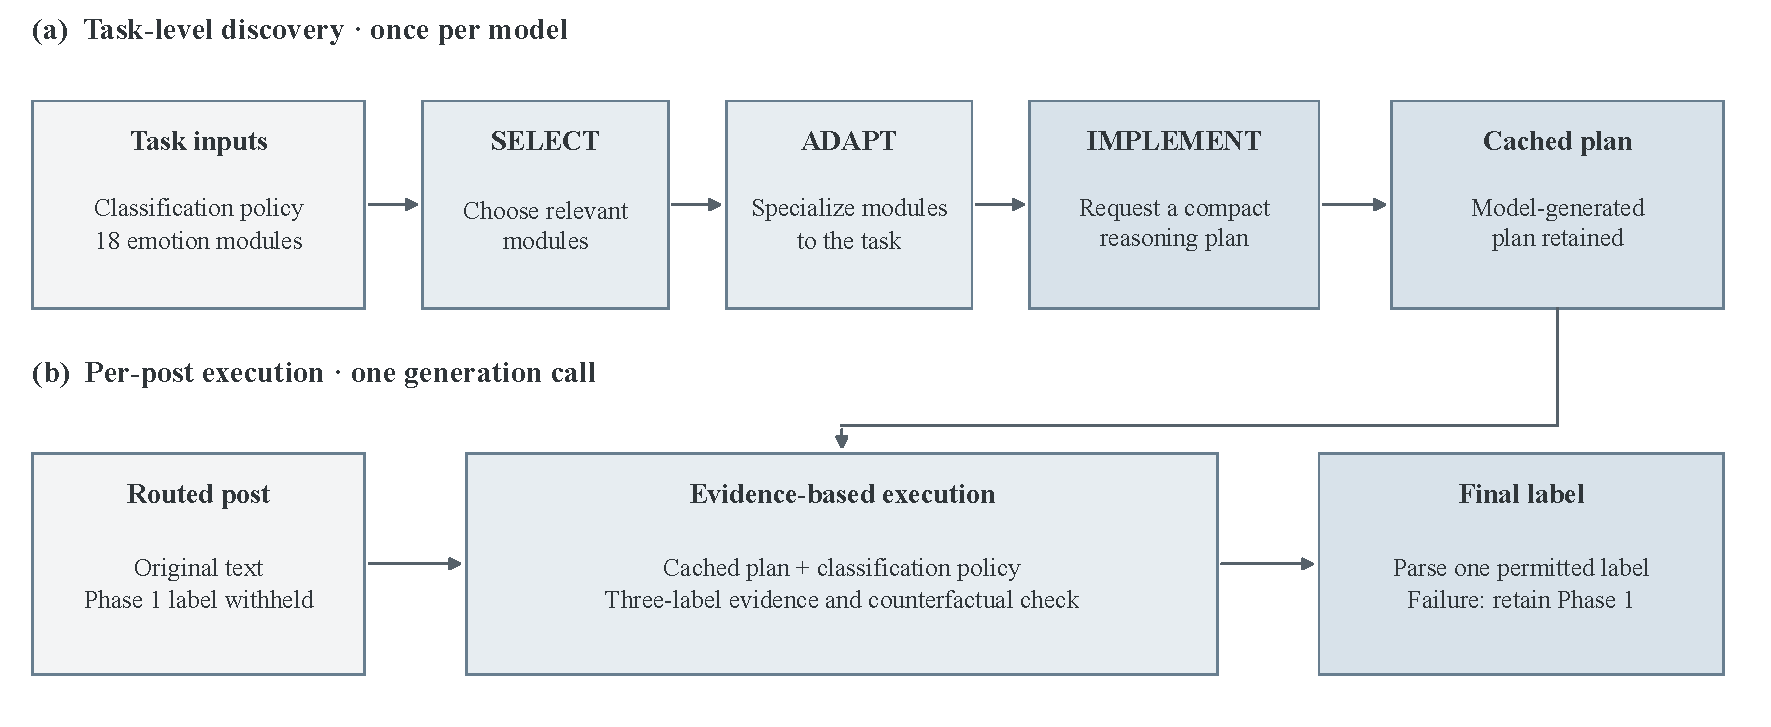
\includegraphics[width=0.96\textwidth]{figures/appendix_sd_workflow.pdf}
\end{center}
\noindent\footnotesize\textbf{Appendix Figure C1.} Final task-level SELF-DISCOVER workflow, separating authorship, timing, and input scope. (a) Researchers supply task materials; before post classification, the selected LLM generates a plan through SELECT, ADAPT, and IMPLEMENT if no retained plan exists. No evaluation post or reference label enters discovery. (b) The same LLM applies the saved plan and fixed researcher-authored checks to each routed original post, generating a fresh response. The dashed arrow denotes plan reuse, not reuse of an answer. Parsing and fallback are code operations, not additional LLM calls.\normalsize\par\medskip

\Needspace{15\baselineskip}\noindent\textsc{Appendix Table C1. Final SELF-DISCOVER stages}\par\smallskip
{\small\renewcommand{\arraystretch}{1.18}
\noindent\begin{tabularx}{\textwidth}{@{}p{0.15\textwidth}YYY@{}}\toprule
Stage & Input & Requested operation & Retained output \\\midrule
SELECT & Task policy and 18 domain modules & Select task-relevant reasoning operations & Selected modules \\
ADAPT & Task description and selected modules & Specialize operations to the three-class task & Adapted modules \\
IMPLEMENT & Adapted modules & Request a compact plan of at most three one-line steps & Actual model-generated plan, cached without a conformance validator \\
Execution & Original post, policy, cached plan & Compare evidence for all three labels and check an alternative interpretation & Response text, parsed label, and failure status \\\bottomrule
\end{tabularx}}\par\medskip

\Needspace{12\baselineskip}
\subsection{Task Description and Module Bank}
\textit{Purpose and scope.} These are researcher-authored inputs to model-level discovery, not an individual evaluation post. The task description defines the three-label annotation problem, and the module bank supplies 18 candidate operations concerning emotional subject, time frame, trajectory, topic, and competing evidence. The policy placeholder expands to the shared classification policy in Appendix~B. The title--body wording is retained verbatim in the Mixed Emotion run, whose supplied input is the synthetic post text.
\lstinputlisting{prompts/sd_task.txt}
\lstinputlisting{prompts/sd_modules.txt}
\Needspace{12\baselineskip}
\subsection{SELECT}
\textit{Input:} the task description and full module bank. \textit{Output:} the model's selected module descriptions, passed to ADAPT. This selection occurs during plan construction, not separately for each evaluated post. Placeholder spelling, including \texttt{resonining\_modules}, is retained from the code.
\lstinputlisting{prompts/sd_select.txt}
\Needspace{12\baselineskip}
\subsection{ADAPT}
\textit{Input:} the task description and SELECT output. \textit{Output:} task-specialized module descriptions, passed to IMPLEMENT. This step asks the model to translate the selected operations into the emotion-classification setting; it does not yet assign a post-level label.
\lstinputlisting{prompts/sd_adapt.txt}
\Needspace{12\baselineskip}
\subsection{Compact IMPLEMENT}
\textit{Input:} the task description and ADAPT output. \textit{Output:} a reusable reasoning plan, retained for later execution. Here IMPLEMENT means constructing the procedure, not executing it on every post. The prompt requests at most three one-line steps and access to the full post at each step. There is no conformance validator or retry enforcing those requests; the realized plans are reported below.
\lstinputlisting{prompts/sd_implement.txt}
\Needspace{12\baselineskip}
\subsection{Per-Post Execution}
\textit{Input:} one routed original post, the shared policy, the model's saved plan, and the fixed execution instructions below. \textit{Output:} a newly generated response ending in a classification line. The system message precedes the user message; \texttt{structure} is replaced by the saved plan and \texttt{text} by this post. No Phase~1 label is supplied to the model.

The evidence ledger is a three-way comparison: for each label the model is asked to identify the strongest supporting and opposing quotation. The subsequent counterfactual check evaluates a competing interpretation rather than changing the post. These are explicit instructions attached to every execution call, not properties guaranteed by caching or by the discovered plan alone.
\lstinputlisting{prompts/sd_system.txt}
\lstinputlisting{prompts/sd_execute.txt}

\Needspace{15\baselineskip}
\subsection{Illustrative Passage Through the Execution Stage}
Consider the constructed sentence, ``Last year I felt isolated; now I enjoy meeting my friends again and feel relieved.'' This is an explanatory example, not a dataset record, model response, or additional evaluation result. The same cached plan would be inserted regardless of this sentence's eventual label. A policy-consistent reading would separate past isolation from current relief, use the quoted time markers as evidence, and examine whether unresolved current distress is actually stated. Under the stated policy, the resolved positive trajectory supports Happy. The example illustrates what the instructions request; it does not show that every generated response follows them.

The evaluator then reads the terminal label from the actual response. A permitted label replaces the Phase~1 prediction for this routed post. If no label is parsed, the evaluator retains Phase~1 instead. Unrouted posts never enter this execution stage. The scored prediction is therefore distinct from the generated explanation, and a parsing failure is not automatically a wrong classification.

\Needspace{12\baselineskip}
\subsection{Realized Cached Plans}
The following plans are reproduced from the recorded notebook outputs, not rewritten to make them conform to the instructions. The Mixed Emotion runs explicitly reused the cached plans. Llama~3 produced three evidence-oriented steps plus a separate final step. Llama~2 produced four prose steps and included provisional label assignment inside early steps. These differences show why the requested plan constraints should not be reported as enforced behavior; they do not independently establish the cause of the performance difference.
\par\medskip\noindent\begin{minipage}{\textwidth}
\textbf{Llama 2 generated plan}
\lstinputlisting{prompts/sd_plan_llama2.txt}
\end{minipage}\par\medskip
\par\medskip\noindent\begin{minipage}{\textwidth}
\textbf{Llama 3 generated plan}
\lstinputlisting{prompts/sd_plan_llama3.txt}
\end{minipage}\par\medskip

\subsection{Generation Budget and Failure Handling}
Direct and CoT request 1,024 new tokens per generation call. Final SD execution requests 1,024 for Llama~2 and 1,536 for Llama~3. The SD discovery calls request up to 512 tokens for Llama~2 and 768 for Llama~3. The source uses a shared per-model cache for the task-level structures, allowing reuse across the Reddit and Mixed Emotion runs. The templates specify instructions, not guaranteed instruction compliance. Quantized model loading, model-specific chat formatting, context limits, and call structure are part of the evaluated implementation. A shorter plan instruction does not by itself prove lower measured cost.

Remaining final SD parsing failures are zero for Llama~2 on both sets, two for Llama~3 Reddit, and one for Llama~3 Mixed Emotion. These remain failures and use Phase~1 fallback. No additional model call is added to resolve them in the reported final SD results.
\section{SELF-DISCOVER Design-Variant Comparison}\label{app:sd-variants}
The earlier independent-countercheck variant generated an instance-specific plan using general reasoning modules; the final version uses a domain-oriented task-level plan and an explicit evidence ledger. Both withhold the Phase~1 label. Multiple components change jointly, so this is a design-variant comparison rather than a single-component causal ablation. The earlier variant is not used in the main six-configuration comparison.

\par\medskip\noindent\textsc{Appendix Table D1. Earlier and final SELF-DISCOVER designs}\par\smallskip
{\small\renewcommand{\arraystretch}{1.18}
\noindent\begin{tabularx}{\textwidth}{@{}p{0.20\textwidth}YY@{}}\toprule
Component & Earlier independent-countercheck & Final task-level compact plan \\\midrule
Discovery scope & A plan constructed for each post & A model-specific plan constructed for the task and reused \\
Module bank & General reasoning operations & 18 emotion-oriented operations \\
Execution guidance & Independent assessment and countercheck & Explicit subject/time checks, three-label quotation ledger, and counterfactual check \\
Phase 1 label & Withheld during SD reasoning & Withheld during SD reasoning \\
Evaluation role & Earlier design comparator in this appendix & SELF-DISCOVER condition in the main comparison \\\bottomrule
\end{tabularx}}\par\medskip

\par\medskip\noindent\textsc{Appendix Table D2. Full-set outcomes of the two SD designs}\par\smallskip
{\small\renewcommand{\arraystretch}{1.18}\noindent\begin{tabular*}{\textwidth}{@{\extracolsep{\fill}}llrrrr@{}}\toprule
Dataset & Model & Earlier acc. & Final acc. & Earlier net & Final net \\\midrule
Reddit & Llama 2 & 97.0500\% & 96.9417\% & 16 & 3 \\
Reddit & Llama 3 & 97.1583\% & 97.2000\% & 29 & 34 \\
Mixed Emotion & Llama 2 & 87.6667\% & 89.3333\% & 12 & 17 \\
Mixed Emotion & Llama 3 & 90.3333\% & 92.6667\% & 20 & 27 \\\bottomrule
\end{tabular*}}\par\medskip
\noindent\textit{Table note.} Accuracy uses all 12,000 Reddit posts or all 300 Mixed Emotion examples, not only routed posts. Net denotes corrected minus introduced errors relative to the same final Phase~1 predictions. ``Earlier'' refers only to the independent-countercheck design, not another intermediate compact-plan version. Table~D2 reports observed outcomes, not a paired significance test between the two SD designs.

The final design improves three of these four model--dataset combinations; it does not uniformly dominate the earlier design. Its Llama~3 configuration improves both datasets. The change in input-independent planning also changes the number and scope of discovery calls, so a cost comparison requires measured generation records rather than accuracy alone.

\Needspace{28\baselineskip}
\section{Paired Accuracy Summaries}\label{app:statistics}
Each row asks whether one complete re-evaluation configuration differs from Phase~1 on the same examples. It does not ask whether SD is better than Direct or CoT. ``Change'' is the full-set accuracy difference in percentage points; the interval estimates uncertainty in that difference; exact $p$ compares the numbers corrected and newly harmed; Holm $p$ adjusts the 12 displayed comparisons.

These calculations use the final reported corrected/introduced counts, with all unparseable SD responses left at the implemented Phase~1 fallback. For accuracy change, the paired correctness-difference counts are sufficient for the exact test and paired bootstrap. This does not constitute a new audit of all raw responses, nor a paired SD-versus-CoT significance test. The latter requires matched per-example predictions from both configurations. Intervals are percentile bootstrap intervals in percentage points. Holm adjustment covers all 12 rows below; it does not account for selection over previously explored prompts.

\par\medskip\noindent\textsc{Appendix Table E1. Paired accuracy comparisons with Phase 1}\par\smallskip
{\small\renewcommand{\arraystretch}{1.18}\noindent\begin{tabular*}{\textwidth}{@{\extracolsep{\fill}}lllrrrr@{}}\toprule
Dataset & Model & Protocol & Change (pp) & Paired 95\% CI & Exact $p$ & Holm $p$ \\\midrule
Reddit & Llama 2 & Direct & +0.0750 & [-0.075, 0.225] & 0.3742 & 1.0000 \\
Reddit & Llama 2 & CoT & +0.0083 & [-0.150, 0.167] & 1.0000 & 1.0000 \\
Reddit & Llama 2 & SELF-DISCOVER & +0.0250 & [-0.142, 0.192] & 0.8424 & 1.0000 \\
Reddit & Llama 3 & Direct & +0.1917 & [0.017, 0.367] & 0.0380 & 0.2281 \\
Reddit & Llama 3 & CoT & +0.2333 & [0.075, 0.392] & 0.0061 & 0.0479 \\
Reddit & Llama 3 & SELF-DISCOVER & +0.2833 & [0.117, 0.458] & 0.0015 & 0.0151 \\
Mixed Emotion & Llama 2 & Direct & -7.3333 & [-11.667, -3.000] & 0.0013 & 0.0139 \\
Mixed Emotion & Llama 2 & CoT & -4.6667 & [-9.333, 0.000] & 0.0704 & 0.3520 \\
Mixed Emotion & Llama 2 & SELF-DISCOVER & +5.6667 & [2.333, 9.000] & 0.0015 & 0.0151 \\
Mixed Emotion & Llama 3 & Direct & +5.6667 & [2.000, 9.667] & 0.0060 & 0.0479 \\
Mixed Emotion & Llama 3 & CoT & +1.0000 & [-2.333, 4.333] & 0.7011 & 1.0000 \\
Mixed Emotion & Llama 3 & SELF-DISCOVER & +9.0000 & [5.667, 12.667] & $<0.0001$ & $<0.0001$ \\
\bottomrule\end{tabular*}}\par\medskip

\clearpage
\section{Synthetic Mixed Emotion Dataset Generation Protocol}

\par\medskip
\noindent\textsc{Appendix Table F1. Synthetic Mixed Emotion Dataset generation protocol}\par
\label{tab:appendix-a5-mixed-emotion-protocol}
\smallskip
\small
\setlength{\tabcolsep}{4pt}
\renewcommand{\arraystretch}{1.08}
\noindent\begin{tabularx}{\textwidth}{@{}>{\raggedright\arraybackslash}p{0.20\textwidth}Y@{}}
\toprule
Component & Description \\
\midrule
Purpose & Construct 300 controlled examples spanning mixed or shifting affect and Neutral controls for supplementary stress-test evaluation. \\
Use in pipeline & Not used for Phase 1 training, hyperparameter tuning, or routing-threshold selection; used only for supplementary robustness evaluation. \\
Class balance & Depression = 100, Neutral = 100, Happy = 100. \\
Scenario balance & Seven controlled scenario groups: five 40-example mixed or shifting-emotion groups, a 75-example clear technical/informational Neutral group, and a 25-example mild factual/procedural-ambiguity Neutral group. \\
Scenario types & Blended-emotion co-occurrence; positive-to-distress shift; distress-to-recovery shift; Neutral framing with subtle affect; conflicting cues with a dominant trajectory; clear technical or informational Neutral content; and mild factual or procedural Neutral ambiguity. \\
Label rule & Assign Depression, Neutral, or Happy according to the dominant overall emotional trajectory, not isolated phrases. \\
Exclusion criteria & Exclude explicit diagnosis claims, treatment advice, medication references, crisis language, identifying information, and off-scenario content. Mixed-cue requirements do not apply to the clear Neutral controls. \\
Prompt disclosure & Generation instructions are reproduced below; the version, model, date, and inclusion criteria are recorded here. \\
Generation record & GPT-5; prompt version \texttt{mixed-emotion-stress-test-v2.4-neutral-clear}; final records dated Aug. 7, 2026. \\
Limitations & Synthetic origin, generation-model style bias, and lack of expert annotation. \\
\bottomrule
\end{tabularx}
\par\medskip


\noindent\small\textit{Generation prompt used for synthetic stress-test examples.}\normalsize\par
\smallskip
\noindent
\begingroup\small
Generate synthetic Reddit-style posts for a controlled mixed-emotion stress-test dataset. Use one of three target labels: Depression, Neutral, or Happy. For Depression and Happy examples, include mixed or shifting cues but make the final emotional trajectory clear to a trained reviewer. For Neutral examples, retain low affective intensity: include either technical/informational content or mild factual/procedural ambiguity without sustained distress, relief, accomplishment, or other dominant affect. When multiple emotions occur, the target label must follow the overall message and final takeaway rather than an isolated phrase.
\par\endgroup\medskip
\begingroup\small
For each example, write one realistic post between 60 and 90 words. Do not include explicit diagnosis claims, medication names, therapy claims, suicide, self-harm, crisis language, usernames, URLs, subreddit names, hashtags, or personally identifying information. Avoid duplicated phrasing and avoid making the label obvious through a single keyword. Return structured records with: example identifier, target label, scenario type, primary context, dominant emotional trajectory, text, and brief label rationale.
\par\endgroup

\par\medskip


\EOD
\end{document}
